\chapter{Proceso de configuración y ambiente de simulación}

En este capítulo se presentan los resultados obtenidos; además, se documenta de forma detallada el procedimiento realizado para configurar cada uno del software utilizado, lo anterior debido a que este trabajo también busca funcionar como una guía estructurada que permita la réplica del la implementación desarrollada.

\section{Configuración del Framework de SIL}
La implementación del trabajo se realizó en una computadora portátil modelo \textit{Acer Aspire E5-575}. A continuación se anexan las características físicas más relevantes del hardware utilizado.

\begin{table}
    \centering
    \begin{tabular}{ll}
        \hline
        Parámetro & Descripción\\
        \hline
        \hline
        Procesador & Intel Core i3-7100U; Dual-core 2.40 GHz\\
        Memoria RAM & 12 GB DDR4\\
        Disco duro & 1 TB Toshiba HDD\\
        Coprocesador de gráficos & Intel HD Graphics 620\\
        \hline
        \hline
    \end{tabular}
    \caption{Características técnicas de la laptop Aspire E5-575}
    \label{tab:specs}
\end{table}

La figura \ref{fig:req} muestra con más detalle las características de hardware y software correspondientes a la computadora donde se llevó a cabo el proyecto. 

\begin{figure}[ht]
    \centering
    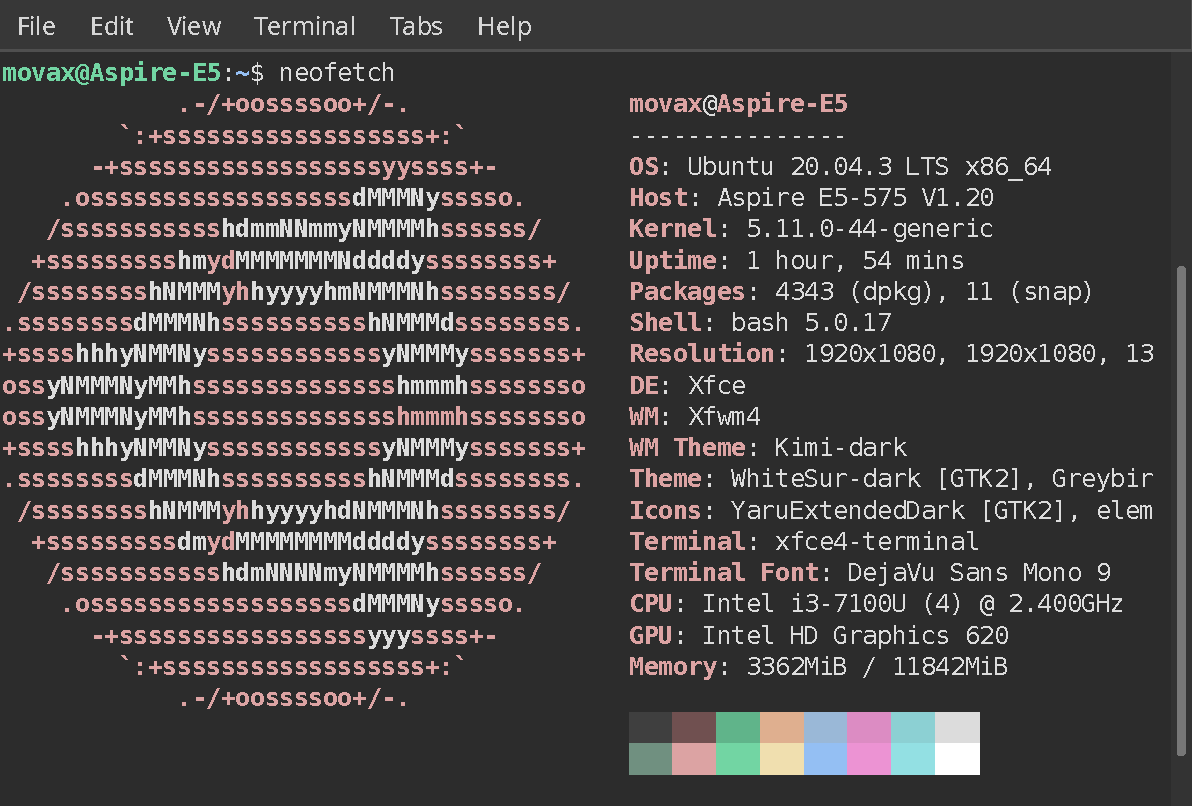
\includegraphics[width=0.6\textwidth]{System_req.pdf}
    \caption{Características del sistema en donde se desarrolló el proyecto}
    \label{fig:req}
\end{figure}

Con respecto al software, se trabajó con las versiones más recientes y técnicamente compatibles del software que integra el sistema. Para el ambiente de simulación se utilizó \textit{Gazebo 11} en conjunto con \textit{ArduPilot} y el modelo ofrecido para SIL de Arducopter; Para la gestión de procesos se utilizó \textit{ROS2 Foxy}. Además, la computadora en donde se implementó el sistema viene por defecto con el sistema operativo \textit{Windows 10}; sin embargo, para poder integrar el software mencionado es necesario utilizar \textit{Ubuntu 20.04.3 LTS (Focal Fossa)}, el cual fue instalado en un disco duro externo.

\subsection{Instalación de ROS 2}
La siguiente serie de comandos fue extraída de la documentación oficial de ROS2 Foxy\cite{ros2} y se asume que la instalación se lleva a cabo en un sistema con Ubuntu 20.04 o sus derivados (\textit{Xubuntu, Kubuntu}, etc.). El proceso puede ser distinto para cualquier otra distribución de Linux o Sistema operativo no listado en la documentación oficial, o incluso puede que no sea compatible.

Cabe destacar que existen dos formas de instalar ROS 2, la primera, la forma corta, es utilizar un paquete binario pre-compilado; sin embargo, este tipo de instalación no incluye la paquetería completa de ROS 2, sino, algunos paquetes base que son más que suficientes para comenzar a desarrollar aplicaciones en ROS. Este primer método puede ser consultado en la documentación oficial de ROS 2 \cite{ROS2Ubuntu}.

Por otro lado, la segunda forma de instalación, la utilizada en este trabajo, corresponde a compilar ROS 2 desde cero en el sistema. A continuación se anexa la serie de comandos y configuración que corresponden a este último método de instalación.


\begin{enumerate}
    \item Revisar que el sistema donde se instalará ROS2 admite la codificación de caracteres \textit{UTF-8}, mediante el siguiente comando.

    \begin{lstlisting}[language = bash]
        $ locale
    \end{lstlisting}

    Sí la codificación se encuentra en la lista, se puede saltar al paso 3, si no, seguir se debe seguir con el resto de pasos.

    \item Instalar la codificación de caracteres

    \begin{lstlisting}[language = bash]
        $ sudo apt update && sudo apt install locales
        $ sudo locale-gen en_US en_US.UTF-8
        $ sudo update-locale LC_ALL=en_US.UTF-8 LANG=en_US.UTF-8
        $ export LANG=en_US.UTF-8
        $ locale #verificacion de instalacion
    \end{lstlisting}

    \item Añadir el repositorio de ROS 2 al sistema. 
    
    \begin{lstlisting}[language = bash]
        $ sudo apt update && sudo apt install curl gnupg2 lsb-release
        $ sudo curl -sSL https://raw.githubusercontent.com/ros/rosdistro/master/ros.key  -o /usr/share/keyrings/ros-archive-keyring.gpg
        $ echo "deb [arch=$(dpkg --print-architecture) signed-by=/usr/share/keyrings/ros-archive-keyring.gpg] http://packages.ros.org/ros2/ubuntu $(lsb_release -cs) main" | sudo tee /etc/apt/sources.list.d/ros2.list > /dev/null
    \end{lstlisting}

    \item Instalar las herramientas de desarrollo para ROS 2

    \begin{lstlisting}[language = bash]
        $ sudo apt update && sudo apt install -y \
          build-essential \
          cmake \
          git \
          libbullet-dev \
          python3-colcon-common-extensions \
          python3-flake8 \
          python3-pip \
          python3-pytest-cov \
          python3-rosdep \
          python3-setuptools \
          python3-vcstool \
          wget
        # Paquetes de Python 3 para pruebas
        $ python3 -m pip install -U \
          argcomplete \
          flake8-blind-except \
          flake8-builtins \
          flake8-class-newline \
          flake8-comprehensions \
          flake8-deprecated \
          flake8-docstrings \
          flake8-import-order \
          flake8-quotes \
          pytest-repeat \
          pytest-rerunfailures \
          pytest
        # Dependencias Fast-RTPS
        $ sudo apt install --no-install-recommends -y \
          libasio-dev \
          libtinyxml2-dev
        # Dependencias Cyclone DDS
        $ sudo apt install --no-install-recommends -y \
          libcunit1-dev
    \end{lstlisting}

    \item Clonar el código fuente de ROS 2

    \begin{lstlisting}[language = bash]
        $ mkdir -p ~/ros2_foxy/src #crea el ambiente de trabajo
        $ cd ~/ros2_foxy
        $ wget https://raw.githubusercontent.com/ros2/ros2/foxy/ros2.repos
        $ vcs import src < ros2.repos
    \end{lstlisting}

    \item Instalar dependencias

    \begin{lstlisting}[language = bash]
        $ sudo rosdep init
        $ rosdep update
        $ rosdep install --from-paths src --ignore-src -y --skip-keys "fastcdr rti-connext-dds-5.3.1 urdfdom_headers"
    \end{lstlisting}

    \item Compilar código fuente
    
    \begin{lstlisting}[language = bash]
        $ cd ~/ros2_foxy/
        $ colcon build --symlink-install
    \end{lstlisting}

    \item Habilitar la API de ROS 2 en bash
    
    \begin{lstlisting}[language = bash]
        $ source /opt/ros/foxy/setup.bash
    \end{lstlisting}

    \item Modificar el perfil de bash para que inicie ROS 2 con cada nueva terminal
    
    \begin{lstlisting}[language = bash]
        $ echo "source /opt/ros/foxy/setup.bash" >> ~/.bashrc 
    \end{lstlisting}

\end{enumerate}

Hecho lo anterior, el sistema debe de contar con una instalación completa de ROS 2. Para comprobar que la instalación se llevó a cabo de manera correcta, se pueden ejecutar los nodos demo que vienen incluidos en la instalación de escritorio.

Para ejecutar los nodos de demostración es necesario abrir dos terminales y ejecutar en cada una uno de los siguientes comandos:

\begin{enumerate}
    \item \textbf{Talker}. Nodo publicador escrito en C++
    \begin{lstlisting}[language = bash]
        $ ros2 run demo_nodes_cpp talker
    \end{lstlisting}
    
    \item \textbf{Listener}. Nodo suscriptor escrito en Python
    \begin{lstlisting}[language = bash]
        $ ros2 run demo_nodes_py listener
    \end{lstlisting}
\end{enumerate}

Las figuras \ref{fig:talker} y \ref{fig:listener} muestran la ejecución de los nodos anteriores, respectivamente. El nodo publicador envía un mensaje con un contador que va incrementando con cada mensaje enviado, mientras que el nodo subscriptor se encarga de recibir el mensaje enviado e imprimirlo en pantalla.

\begin{figure}[ht]
    \centering
    \subfloat[Nodo publicador]{\label{fig:talker}{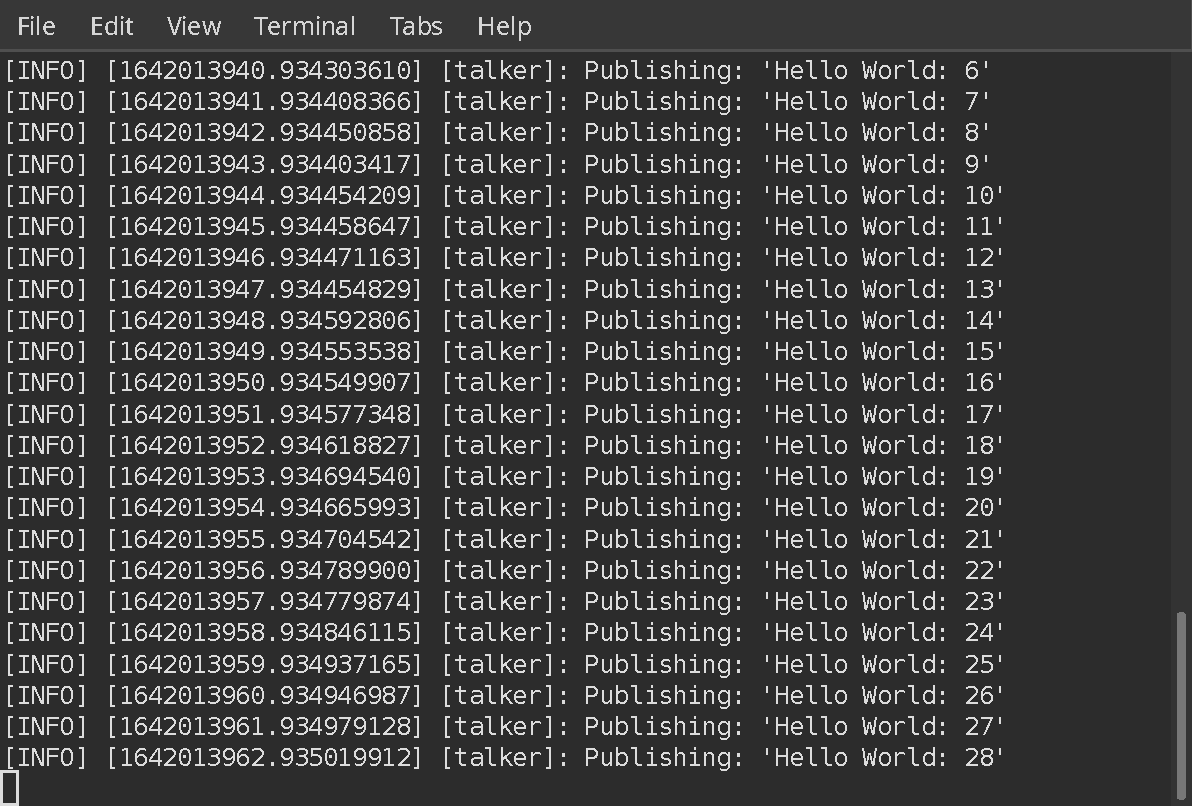
\includegraphics[width=0.48\textwidth]{Talker.pdf}}}\hfill
    \subfloat[Nodos suscriptor]{\label{fig:listener}{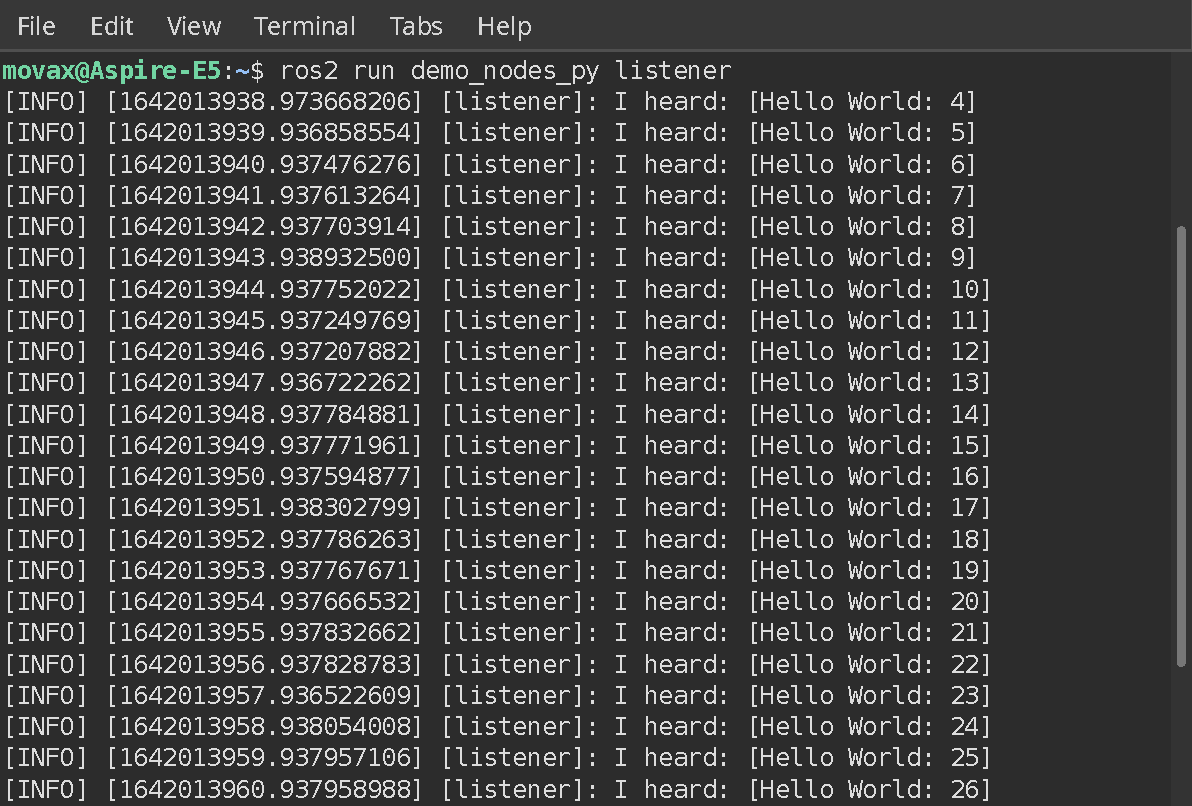
\includegraphics[width=0.48\textwidth]{Listener.pdf}}}
    \caption{Nodos de demostración incluidos en la instalación de ROS 2}
    \label{fig:rosdemo}
\end{figure}

\subsection{Instalación de OpenCV}

Como prerrequisito para instalar la librería de OpenCv es indispensable contar con Python 3 y su gestor de paquetes \textit{pip}. 

La gran mayoría de distribuciones basadas en Ubuntu vienen con Python 3 instalado por defecto. Se puede verificar su instalación con el siguiente comando:

\begin{lstlisting}[language = bash]
    $ python3 --version 
\end{lstlisting}

La expresión anterior debería de imprimir la versión de Python con la que cuenta el sistema, o en su defecto, si Python no se encuentra instalado, se muestra un mensaje que indica que el comando ingresado no existe. Si este último no es el caso, se puede proceder directamente a la instalación de pip.

Instalación de Python 3:
\begin{enumerate}
    \item Actualizar la lista de repositorios del sistema

    \begin{lstlisting}[language = bash]
        $ sudo apt update && sudo apt -y full-upgrade
    \end{lstlisting}
    
    \item Instalar Python 3 desde los repositorios oficiales de Ubuntu

    \begin{lstlisting}[language = bash]
        $ sudo apt install python 3
    \end{lstlisting}

    \item Verificar la instalación de Python

    \begin{lstlisting}[language = bash]
        $ python3 --version 
    \end{lstlisting}

    \item Instalar pip 

    \begin{lstlisting}[language = bash]
        $ sudo apt install python3-pip
    \end{lstlisting}

    \item Verificar instalación de pip

    \begin{lstlisting}[language = bash]
        $ pip3 --version
    \end{lstlisting}
\end{enumerate}

Una vez que se cumplió con el prerrequisito anterior, se puede proceder con la instalación de OpenCV. Cabe mencionar que se aconseja usar ambientes virtuales de Python por cada proyecto, esto con el objetivo de evitar que la instalación de paquetes afecte a otros proyectos desarrollados en el mismo sistema. Sin embargo, debido a que el sistema que utilizado estuvo enfocado exclusivamente a la elaboración de este proyecto, en este trabajo se muestra la instalación global de la librería.

La instalación de la librería es sencilla y se puede realizar con un único comando

\begin{lstlisting}[language = bash]
    $ pip install opencv-contrib-python
\end{lstlisting}

Para verificar la instalación de la librería, se puede ejecutar un pequeño script de Python desde la terminal.

\begin{lstlisting}[language = bash]
    $ python3
    >>> import cv2
    >>> cv2.__version__
\end{lstlisting}

Si la instalación se realizó de forma correcta, se debe de mostrar un mensaje donde se indica la versión de OpenCV que se instaló, como se muestra en la figura \ref{fig:OpenCV_ver}

\begin{figure}[ht]
    \centering
    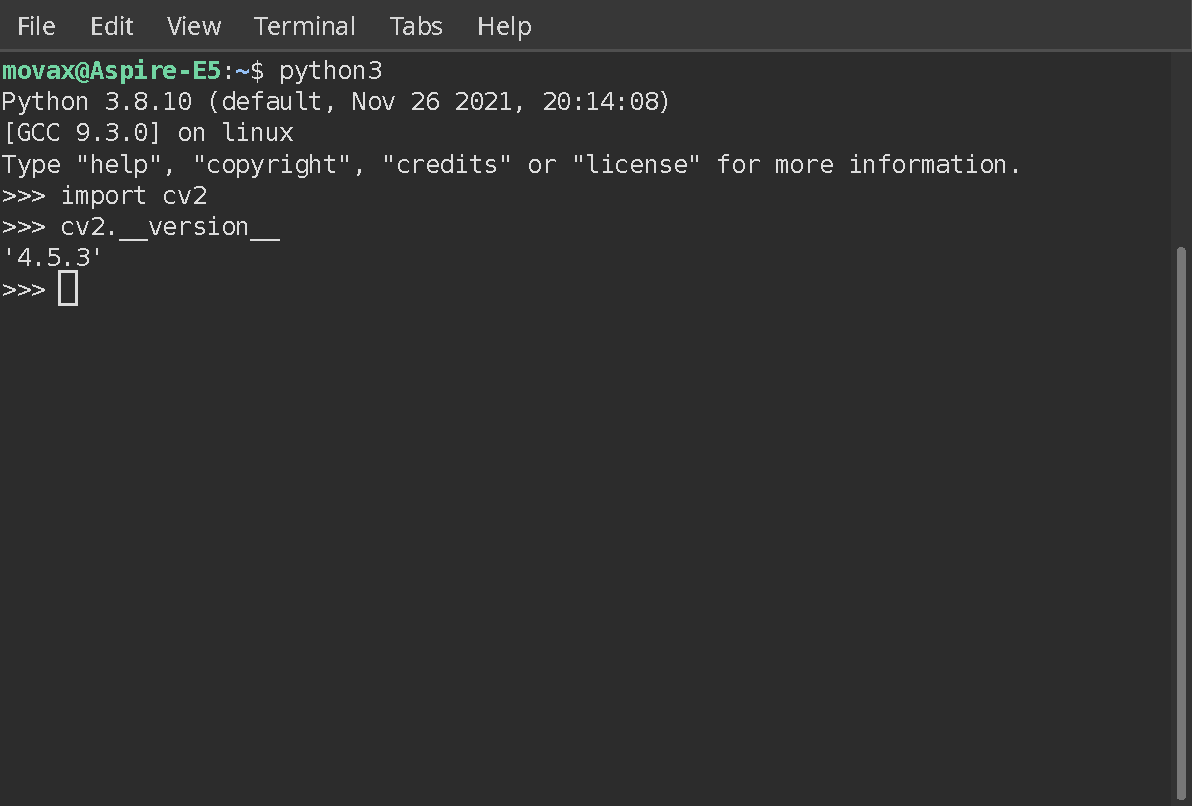
\includegraphics[width=0.6\textwidth]{OpenCV_ver.pdf}
    \caption{Mensaje de validación para la instalación de OpenCV}
    \label{fig:OpenCV_ver}
\end{figure}

\subsection{Instalación de Gazebo}

Como se mencionó en el marco teórico, Gazebo es un ambiente de simulación independiente; es decir, no necesita de ROS o ArduPilot para funcionar. Sin embargo, para habilitar la comunicación entre los nodos de ROS y Gazebo, es recomendable realizar la instalación de Gazebo utilizando los repositorios ofrecidos por ROS 2.

La instalación es sencilla y solo requiere ejecutar el siguiente comando:

\begin{lstlisting}[language = bash]
    $ sudo apt install ros-foxy-gazebo-ros-pkgs
\end{lstlisting}

Al ejecutar la instrucción anterior, se instala en conjunto Gazebo y el plugin para la comunicación entre ROS y Gazebo, \textit{gazebo\_ros\_pkg}. Además, el repositorio también incluye una serie de simulaciones de prueba para demostrar la manera en la que se lleva a cabo la comunicación entre una simulación en Gazebo y un nodo de ROS. 

Por otro lado, cabe destacar que, de la misma forma en la cada versión de ROS es desarrollada para trabajar bajo una versión especifica de Ubuntu, cada versión de ROS también tiene asociada una única versión compatible de Gazebo; para el caso de ROS 2 Foxy, se trabaja con la última versión disponible, Gazebo 11. La figura \ref{fig:Gazebo_ver} muestra los datos técnicos sobre la versión de Gazebo con la que se trabajó.

\begin{figure}[ht]
    \centering
    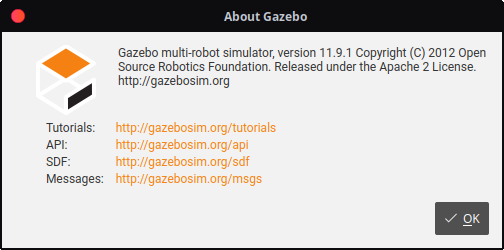
\includegraphics[width=0.5\textwidth]{Gazebo_ver.png}
    \caption{Ficha técnica de la versión de Gazebo}
    \label{fig:Gazebo_ver}
\end{figure}


Una vez que terminó la ejecución del comando anterior, se puede verificar que la instalación se realizó de manera correcta ejecutando Gazebo desde la terminal, tal que

\begin{lstlisting}[language = bash]
    $ gazebo
\end{lstlisting}

La instrucción anterior ejecuta una instancia de Gazebo, en donde al no haber ingresado ningún parámetro para cargar un mundo o ambiente de simulación existente, se abre la pantalla inicial del simulador, con un mundo vacío, tal como se muestra en la figura \ref{fig:Gazebo_world}.

\begin{figure}[ht]
    \centering
    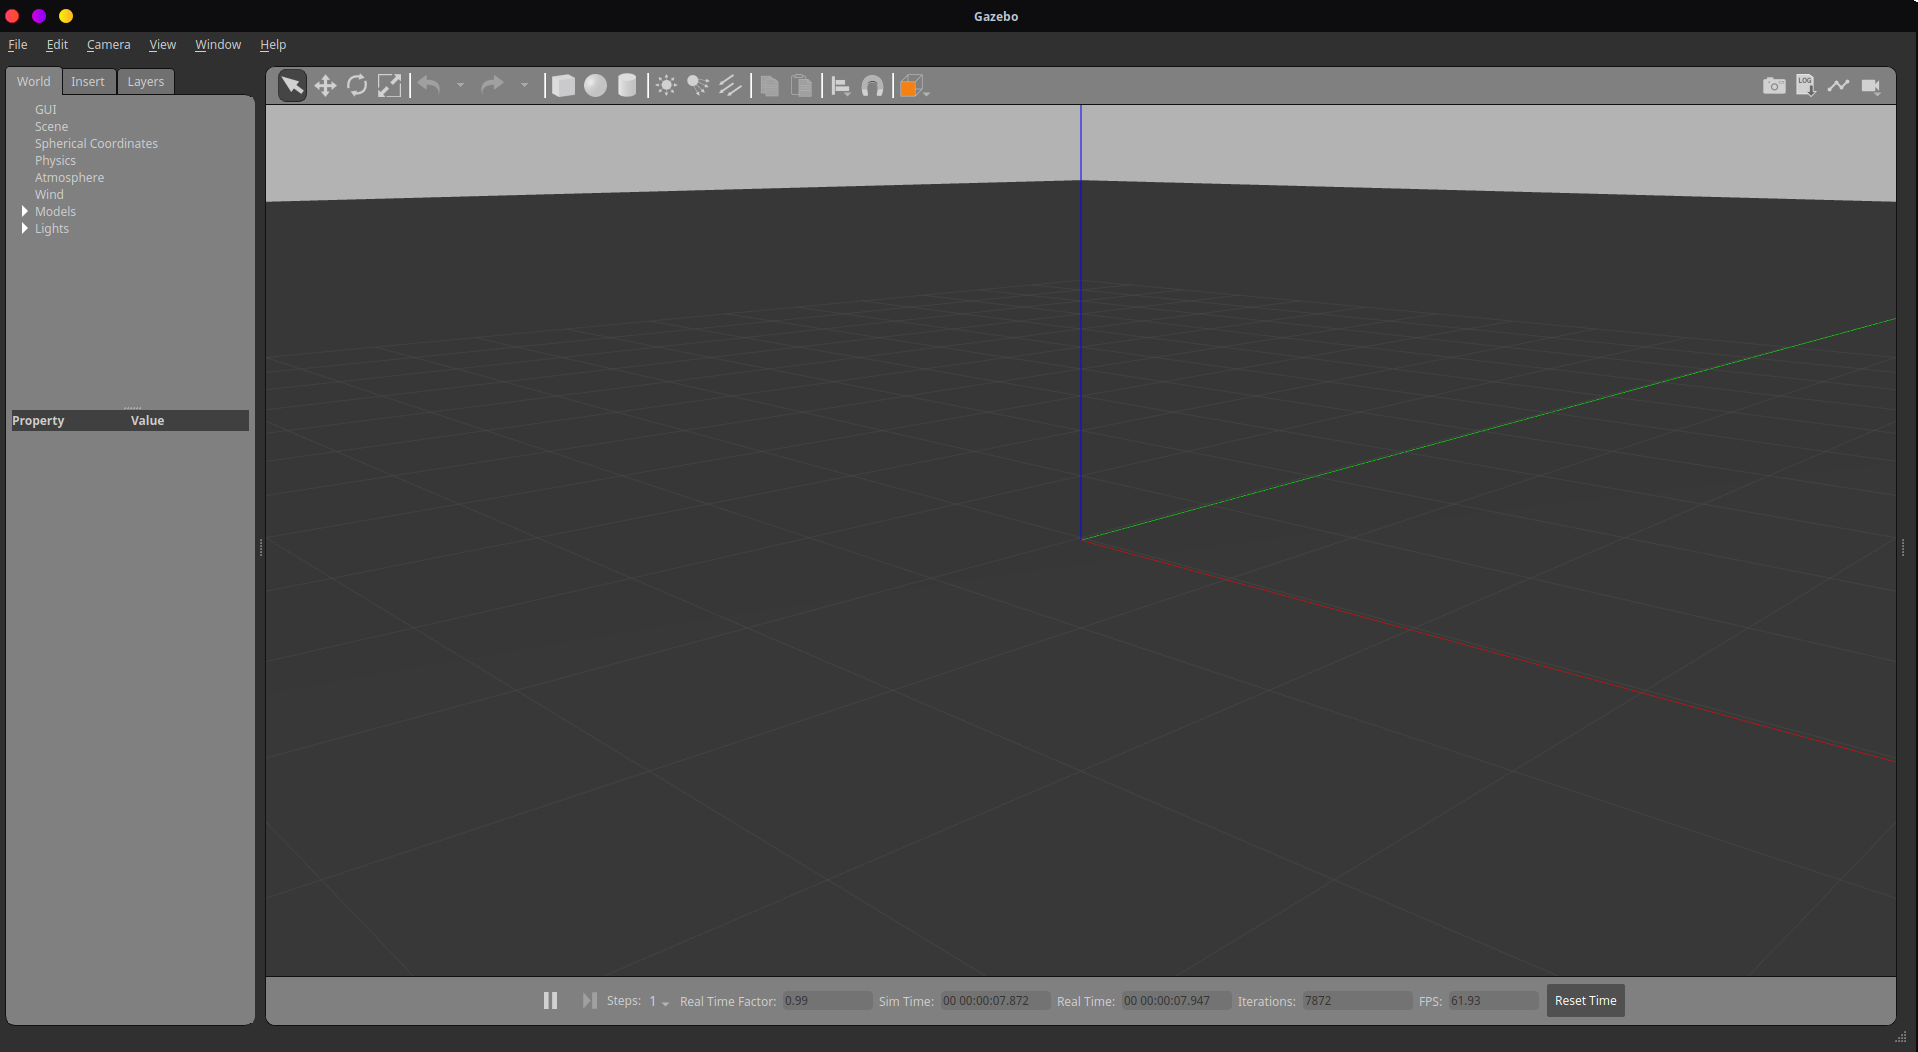
\includegraphics[width=\textwidth]{Gazebo_world.png}
    \caption{Proyecto vacío generado al inicializar Gazebo}
    \label{fig:Gazebo_world}
\end{figure}

Por otro lado, con el fin de comprobar la comunicación entre ROS y Gazebo, se puede ejecutar una de las simulaciones demos incluidas en la instalación. Para ello se selecciona una de las simulaciones más básicas, en donde se tiene un modelo sencillo de un robot y por medio de un topic de ROS se envían instrucciones al robot para su desplazamiento.

Para realizar lo anterior primero se debe de ejecutar una instancia de Gazebo con el mundo que se desea simular.

\begin{lstlisting}[language = bash]
    $ gazebo --verbose /opt/ros/foxy/share/gazebo_plugins/worlds/gazebo_ros_diff_drive_demo.world
\end{lstlisting}

Una vez iniciada la simulación, se pueden enviar instrucciones para el robot por medio de ROS, de la siguiente manera:

\begin{lstlisting}[language = bash]
    $ ros2 topic pub /demo/cmd_demo geometry_msgs/Twist '{linear: {x: 1.0}}' -1
\end{lstlisting}

\begin{figure}[ht]
    \centering
    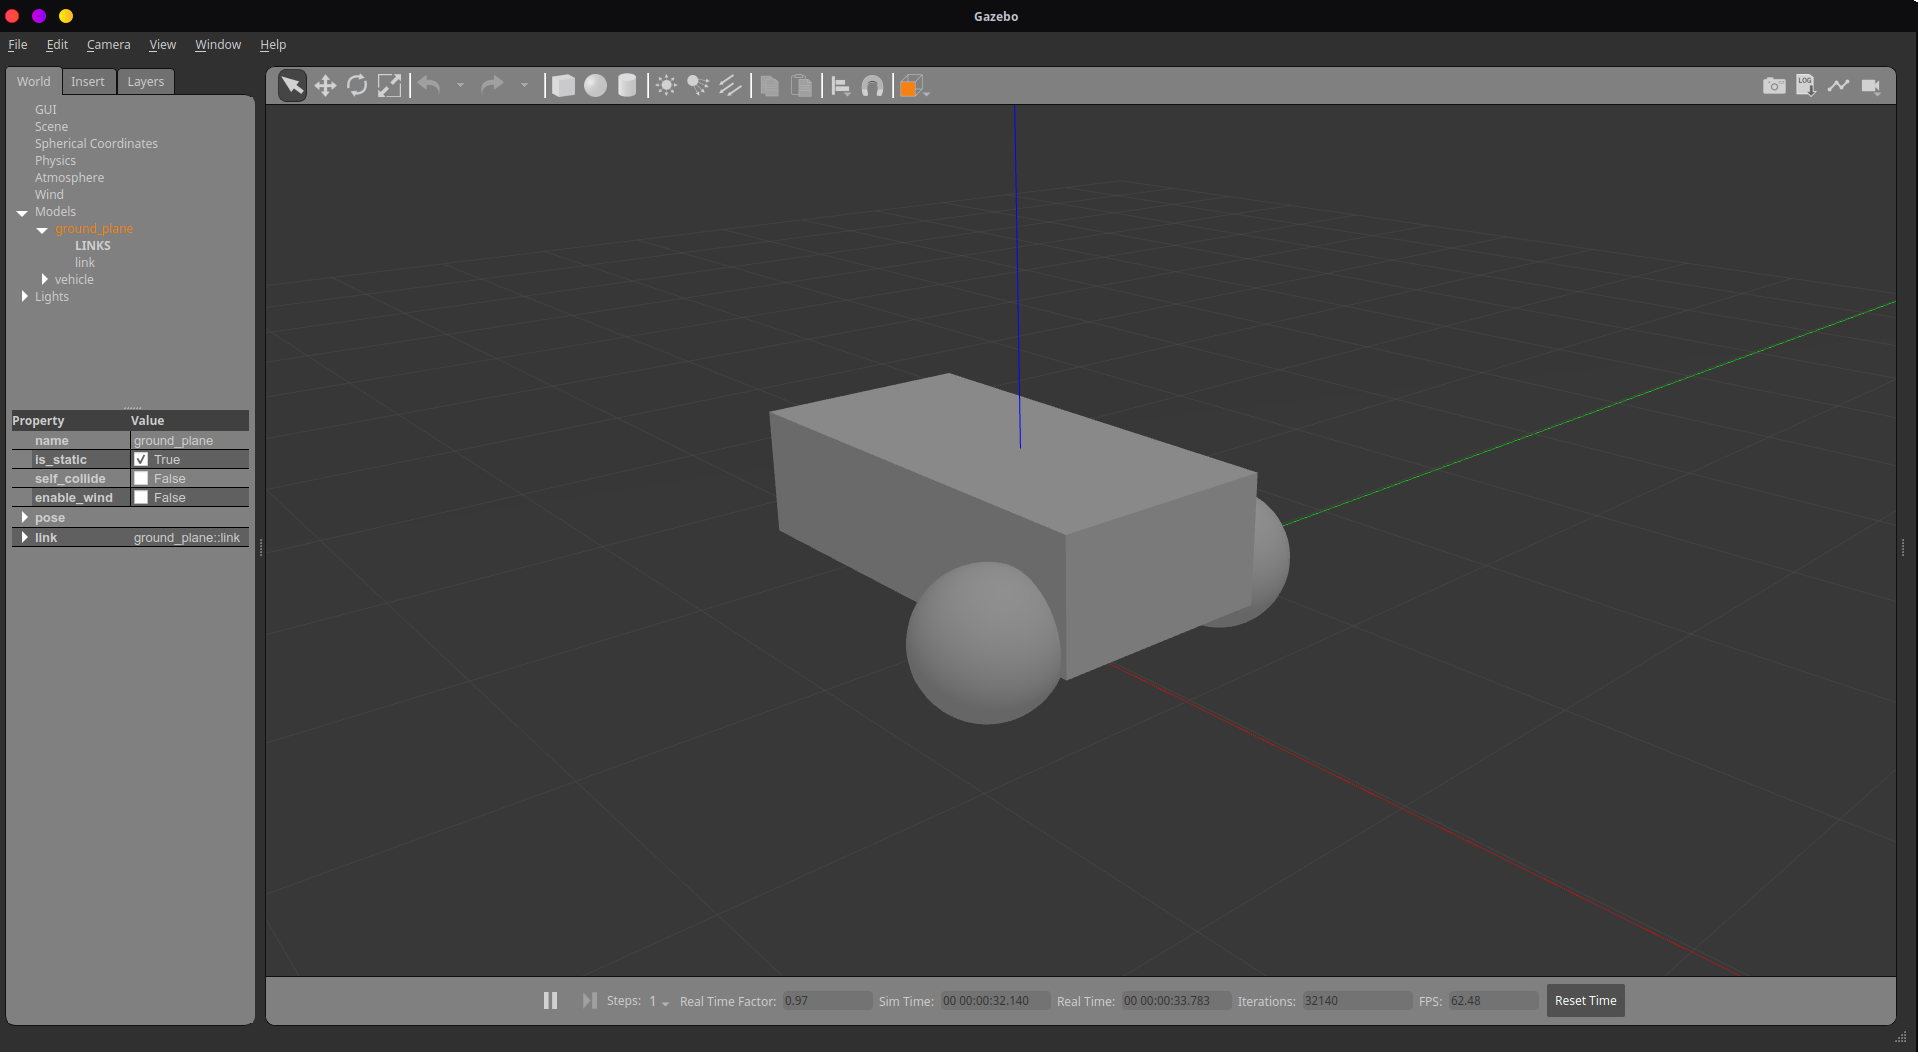
\includegraphics[width=\textwidth]{Gazebo_ros.png}
    \caption{Proyecto de demostración en Gazebo que incluye el plug-in para comunicarse con ROS}
    \label{fig:Gazebo_ros}
\end{figure}

La figura \ref{fig:rossims} muestra el movimiento observado en la simulación  a partir de haber ingresado un comando por medio de la API de ROS.

\begin{figure}[ht]
    \centering
    \subfloat[Primera posición]{\label{fig:rossim1}{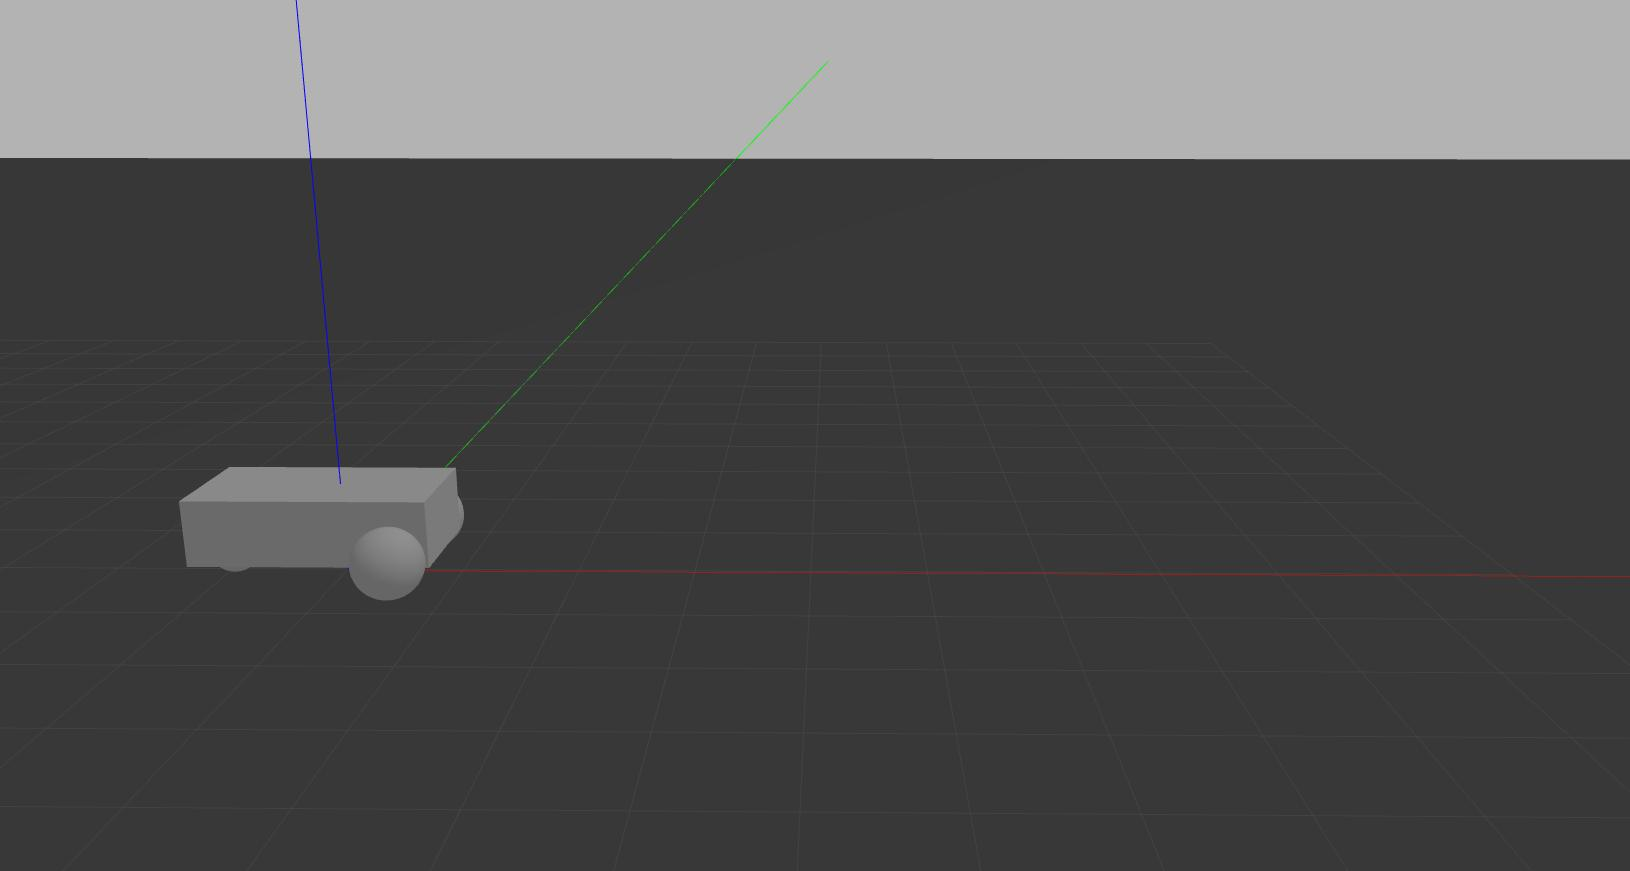
\includegraphics[width=0.48\textwidth]{ROS_sim1.jpg}}}\hfill
    \subfloat[Segunda posición]{\label{fig:rossim2}{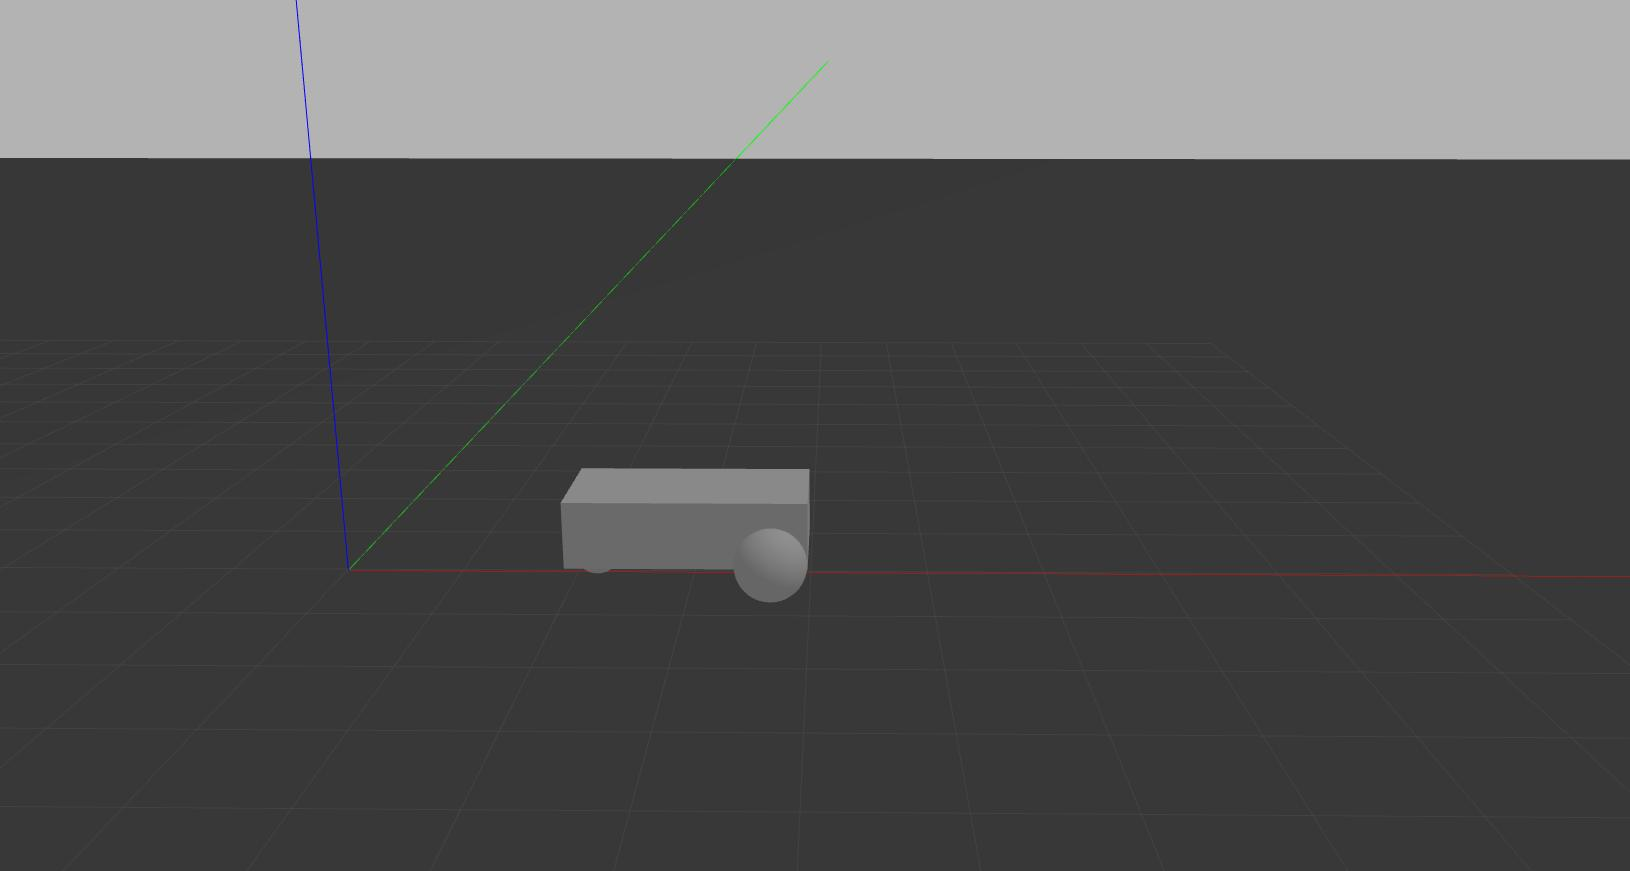
\includegraphics[width=0.48\textwidth]{ROS_sim2.jpg}}}\\
    \subfloat[Tercera posición]{\label{fig:rossim3}{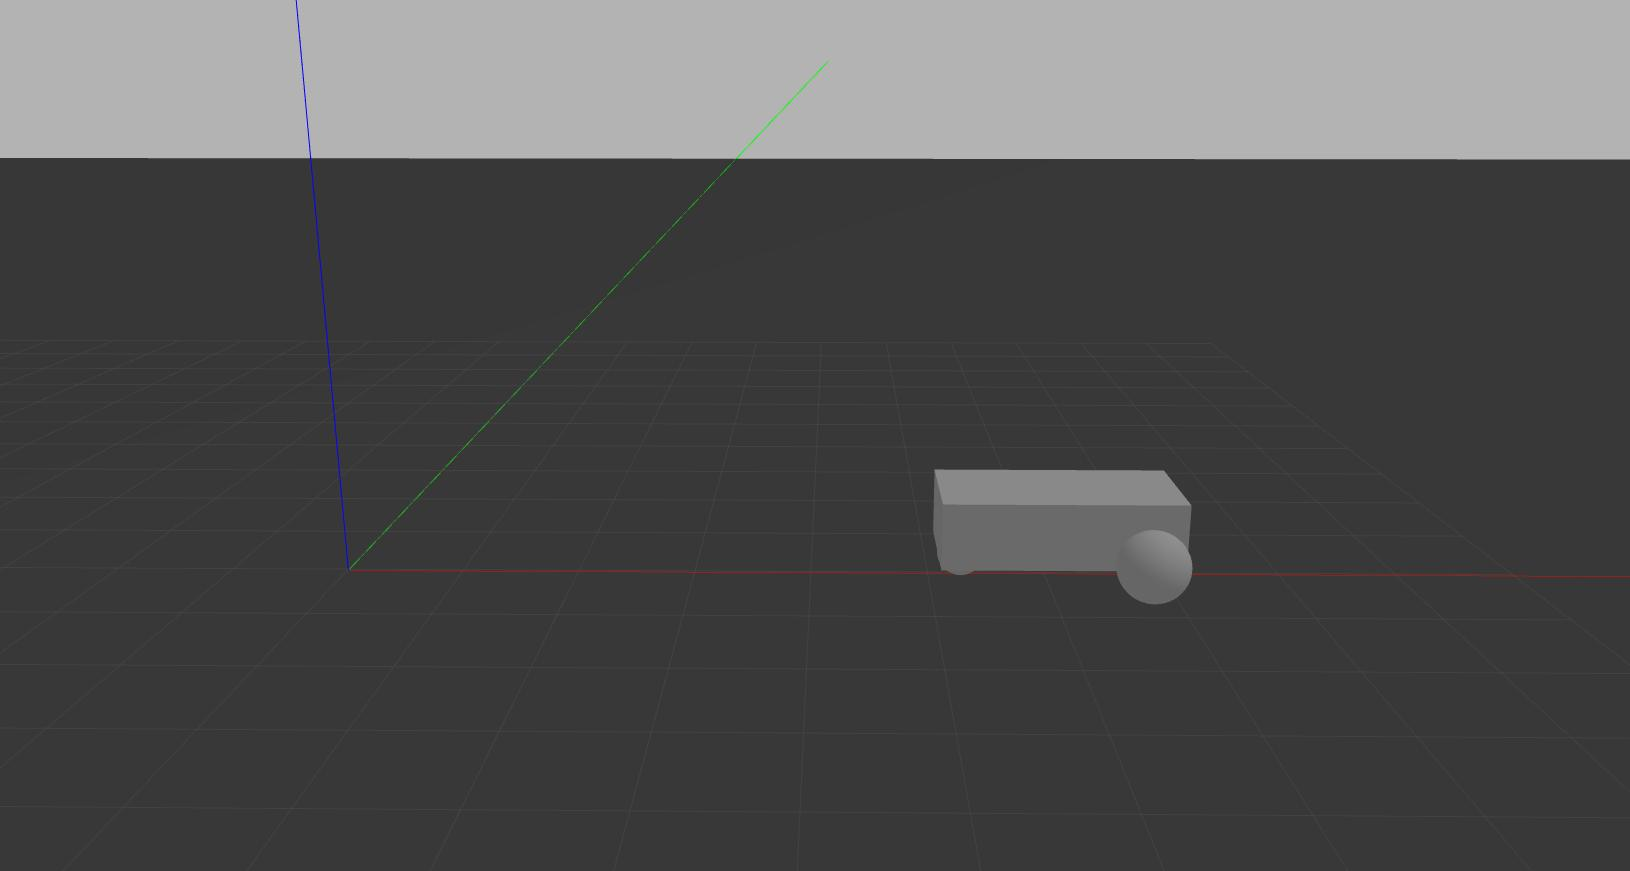
\includegraphics[width=0.48\textwidth]{ROS_sim3.jpg}}}\hfill
    \subfloat[Cuarta posición]{\label{fig:rossim4}{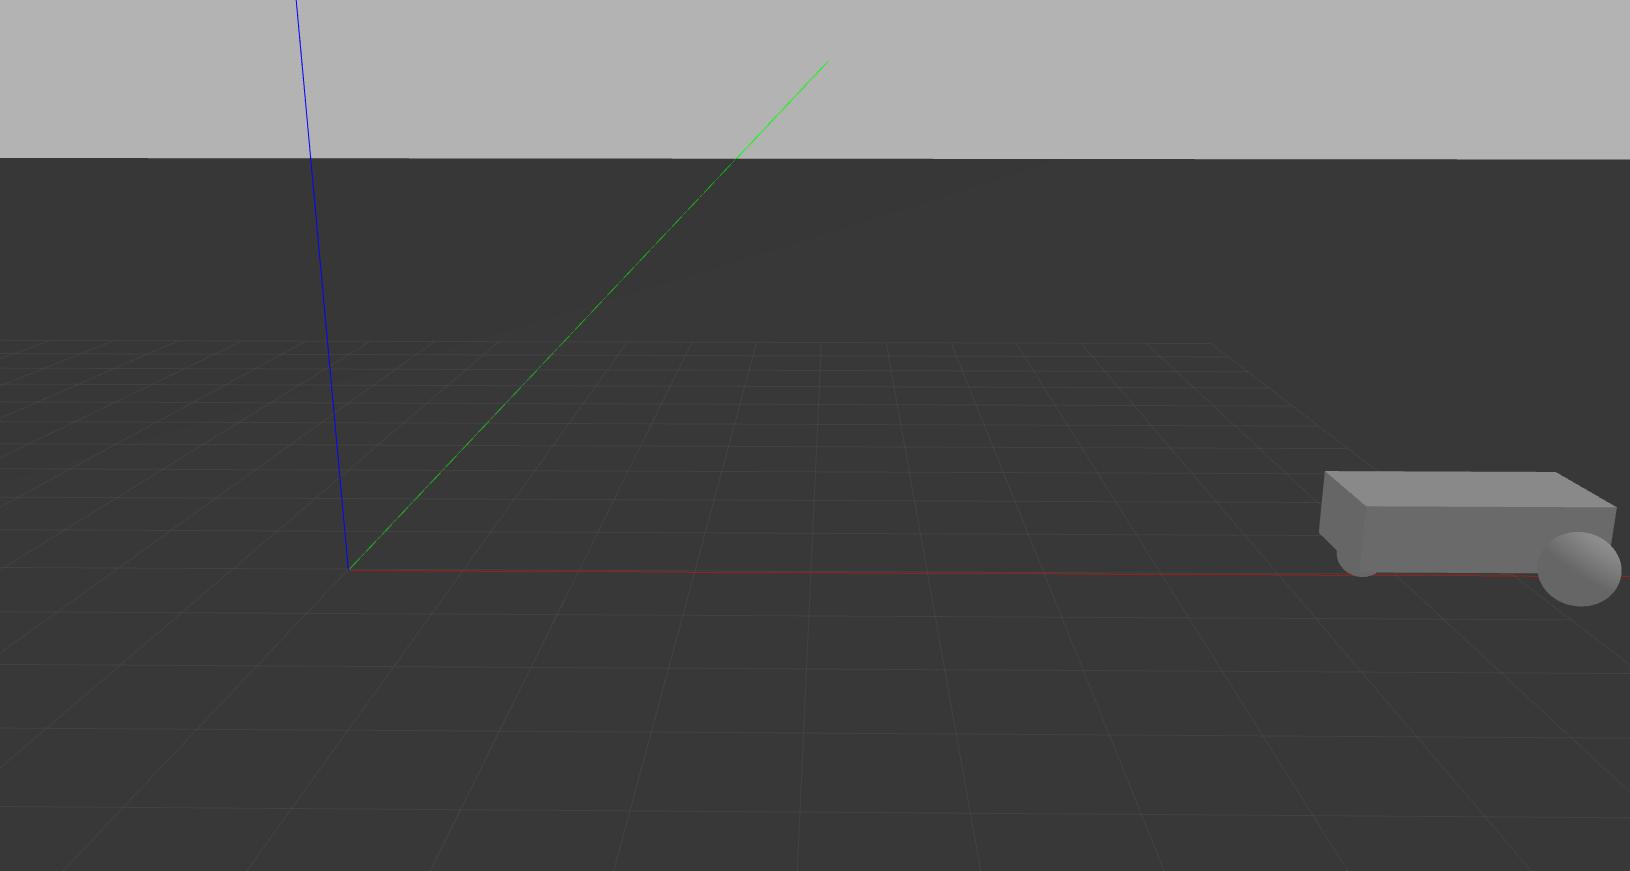
\includegraphics[width=0.48\textwidth]{ROS_sim4.jpg}}}
    \caption{Movimiento de la simulación en Gazebo con plugin de comunicación de ROS}
    \label{fig:rossims}
\end{figure}


Para consultar el resto de simulaciones de demostración incluida, se puede acceder al directorio donde se encuentra instalado ROS y listar los nombre de las simulaciones instaladas. Es posible abrir los archivos de simulación con un editor de texto y observar la documentación incluida en cada una, en donde se especifica el modo de uso de esta, la interfaz de mensajes que utilizar para la comunicación y la sintaxis necesaria para enviar mensajes utilizando ROS.

\begin{lstlisting}[language = bash]
    $ cd  /opt/ros/foxy/share/gazebo_plugins/worlds
    $ ls 
\end{lstlisting}

\begin{figure}[ht]
    \centering
    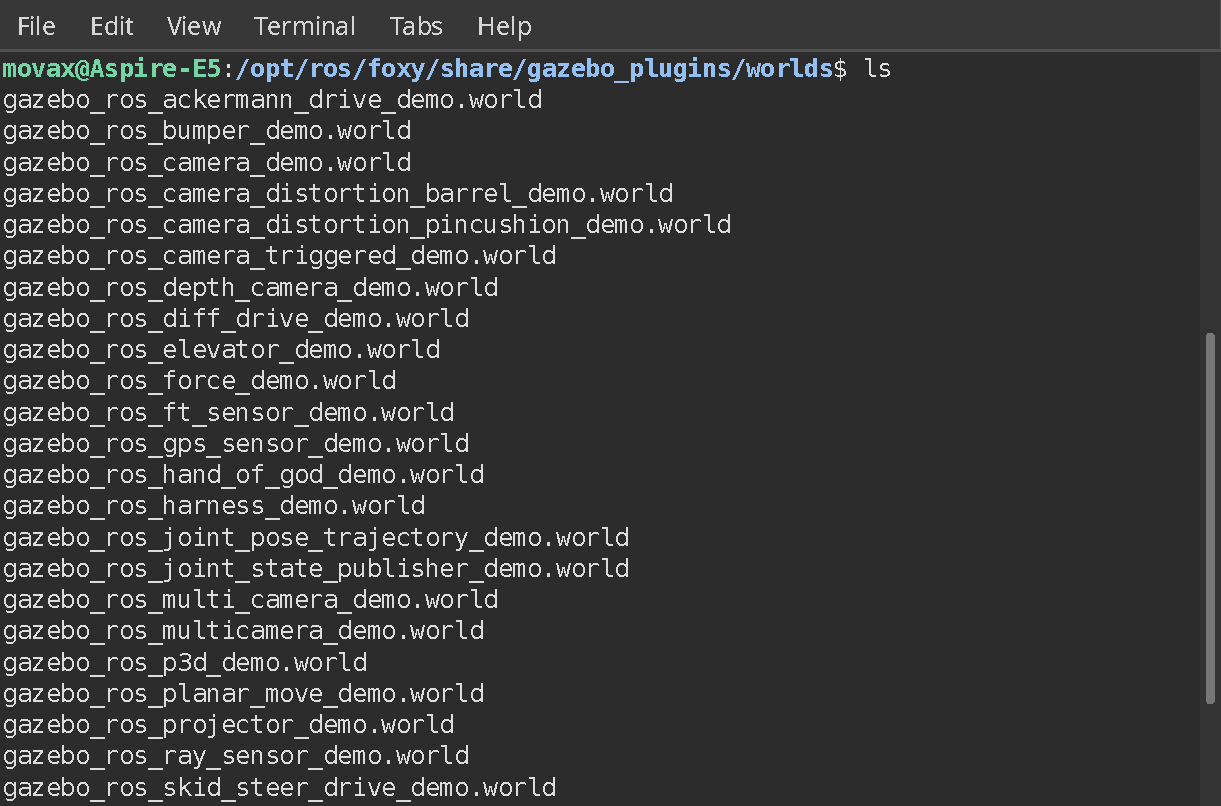
\includegraphics[width=0.6\textwidth]{ROS_demos.pdf}
    \caption{Lista de simulaciones de demostración para el uso de Gazebo con ROS 2}
    \label{fig:ROS_demos}
\end{figure}

\subsection{Instalación de ArduPilot SIL Simulator}
Configurar y trabajar con el framework de simulación de ArduPilot es quizás la parte más compleja en cuanto al software utilizado para el sistema propuesto. Esto es debido a que la gran parte de la documentación oficial se encuentra desactualizada y los recursos que proveen información al respecto se encuentran dispersos por foros y otros tipos de documentación no oficial. 

A continuación se muestra una síntesis del proceso de instalación y Configuración para ArduPilot SIL Simulator.

\begin{enumerate}

    \item Ubicarse en el directorio donde se desean almacenar los archivos del repositorio de ArduPilot y clonar el proyecto.

    \begin{lstlisting}[language = bash]
        $ git clone --recursive https://github.com/ArduPilot/arduPilot.git
        $ cd arduPilot
    \end{lstlisting}    

    \item Instalar las herramientas necesarias para la compilación de ArduPilot
    
    \begin{lstlisting}[language = bash]
        $ Tools/environment_install/install-prereqs-ubuntu.sh -y
    \end{lstlisting}   

    \item Recargar la ruta de trabajo para hacer uso de las herramientas
    
    \begin{lstlisting}[language = bash]
        $ . ~/.profile
    \end{lstlisting}   

    \item Compilar el paquete seleccionando el modelo de computadora de vuelo y el vehículo deseado.

    \begin{lstlisting}[language = bash]
        $ ./waf configure --board CubeBlack
        $ ./waf copter
    \end{lstlisting}

    Como comentario complementario, ArduPilot es compatible con varios modelos de computadoras de vuelo, en este caso se seleccionó una \textit{Pixhawk2 Cube}. Para obtener el listado de todas las computadoras de vuelo compatibles, se puede ejecutar la siguiente instrucción; de tal forma que es posible seleccionar cualquier otro modelo cambiando el nombre del parámetro por cualquier de la lista. 

    \begin{lstlisting}[language = bash]
        $ ./waf list_boards
    \end{lstlisting}

    De igual manera, el parámetro de vehículo puede ser modificado por el nombre de otro de los vehículos con los que trabaja ArduPilot, acorde a las necesidades del usuario. Para enlistar los vehículos disponibles se puede utilizar el comando \textit{"list"}.
    
    \begin{lstlisting}[language = bash]
        $ ./waf list
    \end{lstlisting}

    \item Limpiar los archivos temporales generados tras la compilación.
    
    \begin{lstlisting}[language = bash]
        $ ./waf clean
    \end{lstlisting}

    \item Añadir el API de ArduPilot al perfil de bash
    
    \begin{lstlisting}[language = bash]
        $ echo "export PATH=$PATH:$HOME/ardupilot/Tools/autotest" >> ~/.bashrc
        $ echo "export PATH=/usr/lib/ccache:$PATH" >> ~/.bashrc 
    \end{lstlisting}  

    \item Recargar el directorio de trabajo con el nuevo perfil de bash
    
    \begin{lstlisting}[language = bash]
        $ . ~/.bashrc
    \end{lstlisting}  

\end{enumerate}

Hecho lo anterior, se puede realizar la prueba del  framework de SIL, para ello es necesario dirigirse al directorio del vehículo instalado, dentro del directorio donde se descargó ArduPilot. 

\begin{lstlisting}[language = bash]
    $ cd ~/ardupilot/ArduCopter
\end{lstlisting}  

Una vez dentro del directorio, se puede ejecutar la simulación del vehículo con el siguiente comando:

\begin{lstlisting}[language = bash]
    $ sim_vehicle.py --map --console
\end{lstlisting}  


El comando anterior ejecuta una instancia del SIL de ArduPilot, de tal forma que se abren dos ventanas; un mapa una terminal.

La terminal que se abre al momento de ejecutar la simulación corresponde a la consola de vuelo, en esta se indican algunos parámetros de interés del dron, tal como el nivel de la batería, el modo de vuelo, la altura a la que se encuentra, un historial de eventos, entre otras cosas.

El mapa contiene un pequeño esquema de un cuadricóptero (vehículo compilado para este trabajo) y es donde se puede observar su desplazamiento con base en los comandos ingresados a partir de la terminal de ArduPilot.

Es posible controlar el dron utilizando comandos ingresados desde la terminal o directamente utilizando el mapa. Es posible asignar waypoints y rutas de vuelo de forma gráfica dando clic derecho sobre el mapa.

A continuación se adjuntan una serie de comandos ejemplo para realizar un desplazamiento básico, en donde el dron despega 10 m sobre el suelo y luego se mueve otros 20 m en el eje x.

Se debe de ingresar lo siguiente en la terminal desde donde se inició la sesión de ArduPilot:

\begin{lstlisting}[language = bash]
    > mode guided     #cambia el modo de vuelo
    > arm throttle    #arma los motores del dron
    > takeoff 10      #despegue
    > position 50 0 0 #desplazamiento en x,y,z
\end{lstlisting}  

Lo anterior corresponde a una demostración del uso básico del simulador standalone de ArduPilot; sin embargo, en este trabajo se propone Gazebo como ambiente de simulación, por lo que es necesario conectar el SIL de Ardupilot con este simulador. Lo anterior es posible realizando la instalación de un plugin específicamente diseñado con este propósito.


\begin{figure}[ht]
    \centering
    \subfloat[Posición inicial]{\label{fig:Ardupilot_gc}{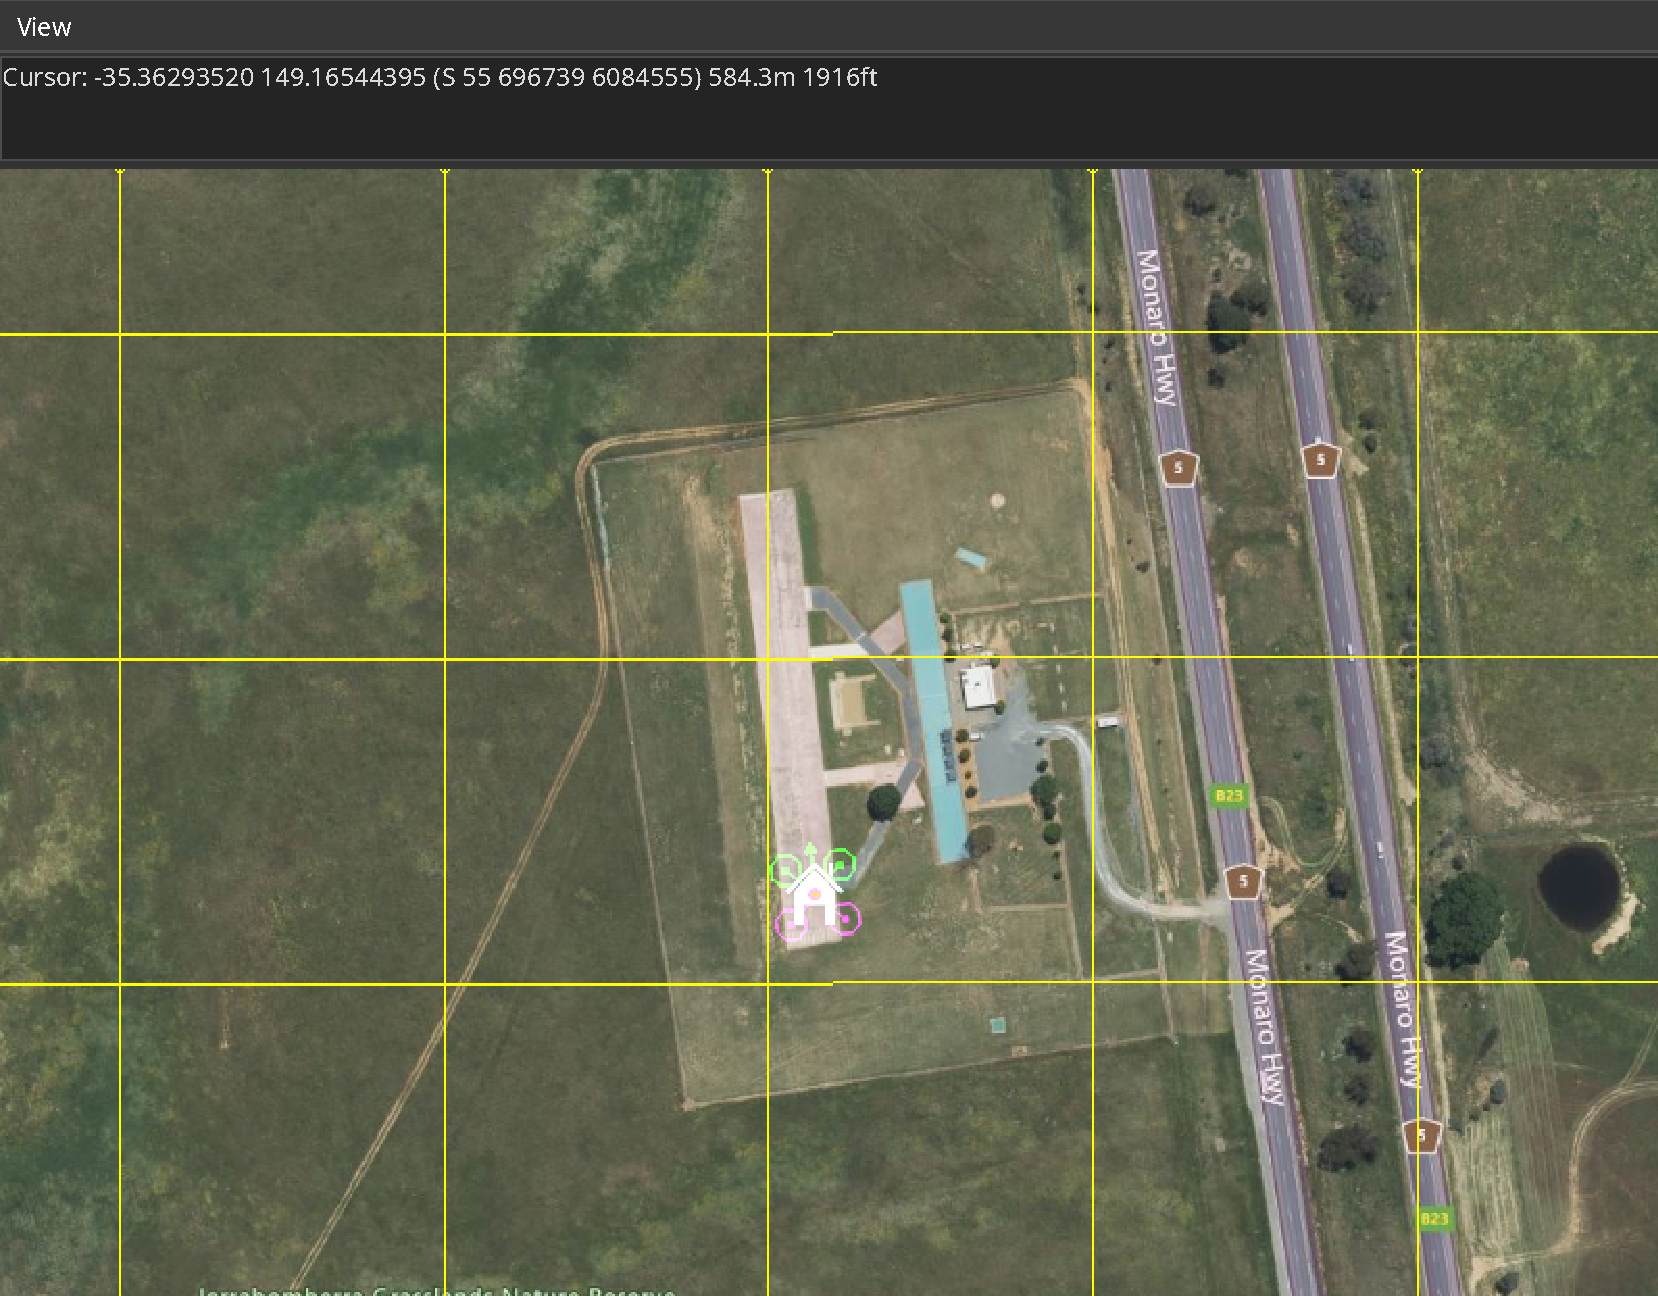
\includegraphics[width=0.48\textwidth]{Ardupilot_gc.pdf}}}\hfill
    \subfloat[Posición final]{\label{fig:Ardupilot_gc1}{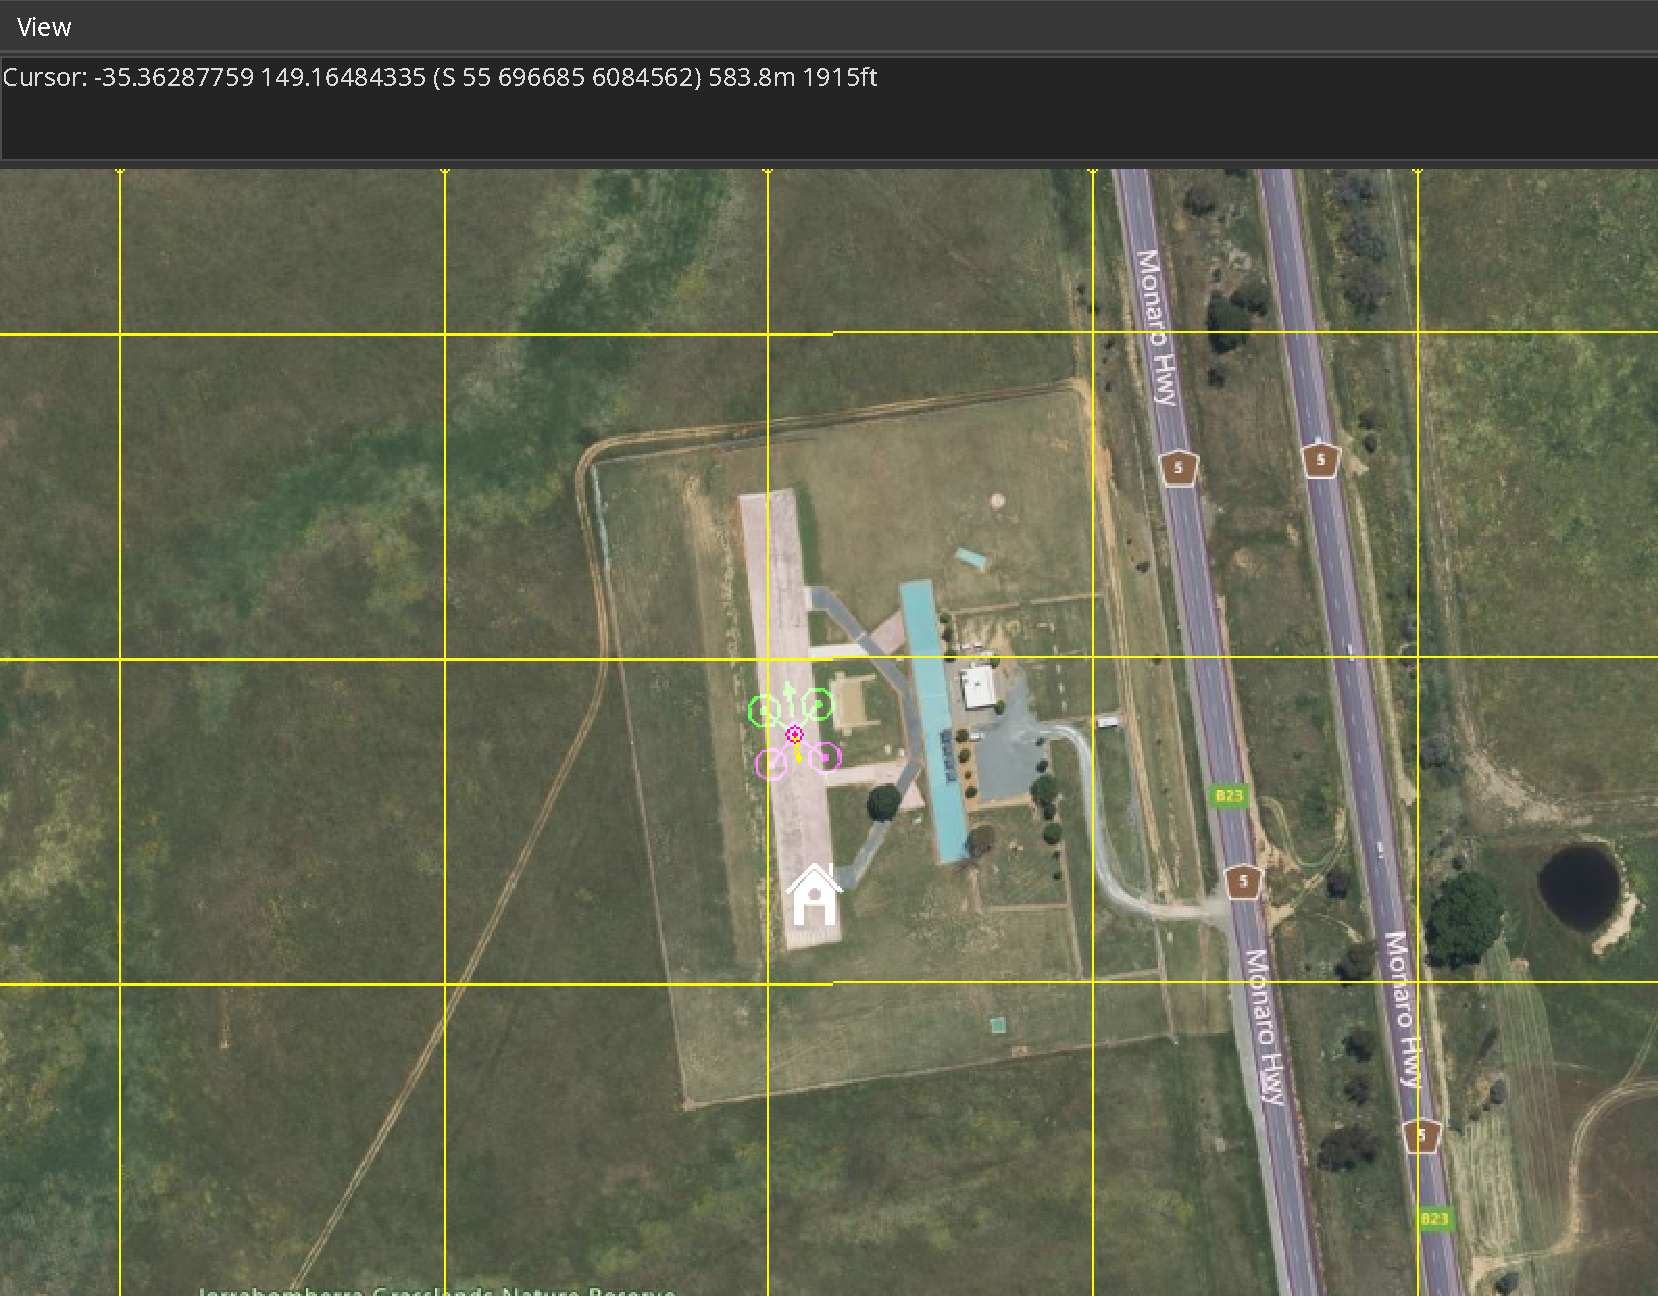
\includegraphics[width=0.48\textwidth]{Ardupilot_gc1.pdf}}}\\
    \subfloat[Terminal con comando de vuelo]{\label{fig:Ardupilot_gcterminal}{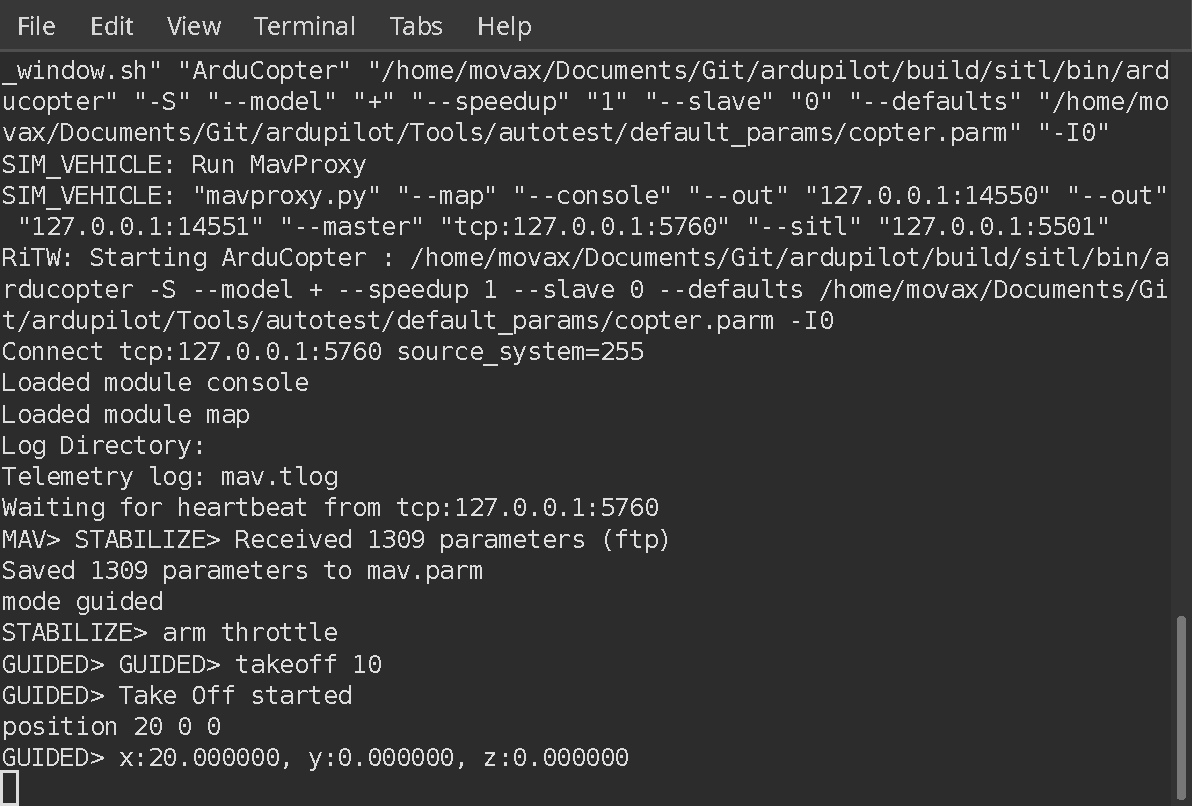
\includegraphics[width=0.5\textwidth]{Ardupilot_gcterminal.pdf}}}\hfill
    \caption{Prueba de ejecución del framework de SIL de ArduPilot}
    \label{fig:Ardupilot}
\end{figure}

\begin{figure}[ht]
    \centering
    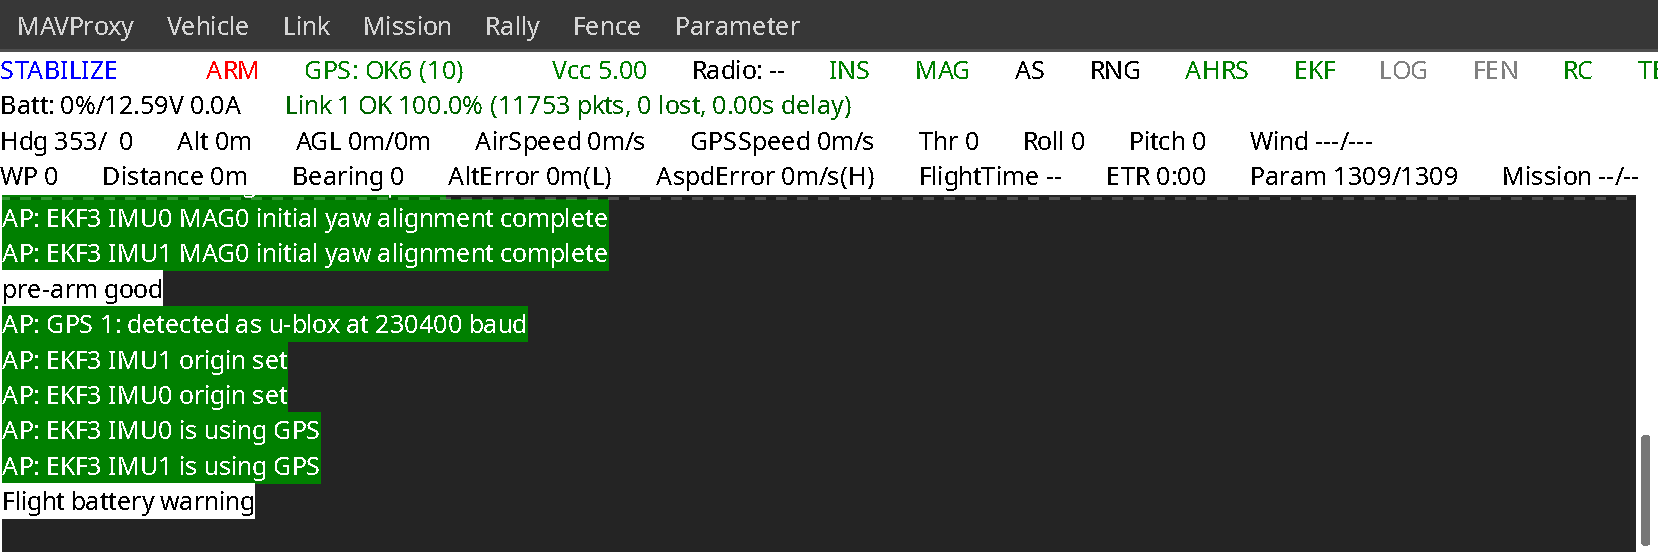
\includegraphics[width=0.8\textwidth]{Ardupilot_mavproxy.pdf}
    \caption{Terminal de información del sistema de ArduPilot}
    \label{fig:Ardupilot_mavproxy}
\end{figure}

\begin{figure}[ht]
    \centering
    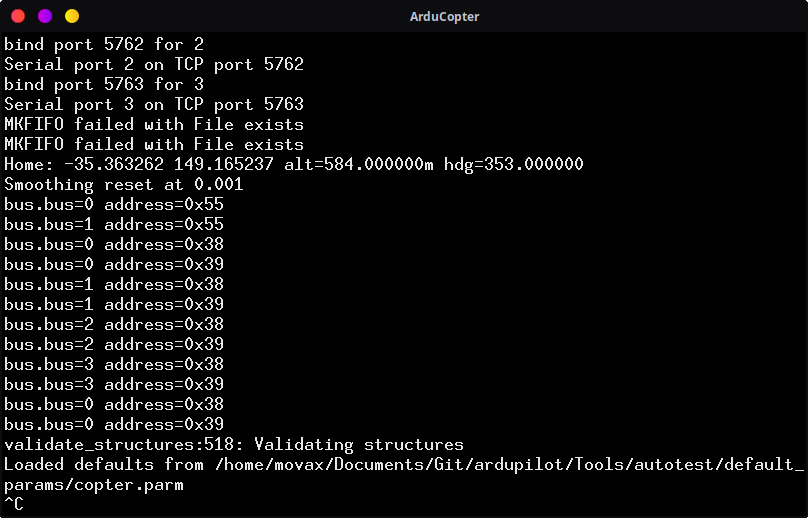
\includegraphics[width=0.8\textwidth]{Ardupilot_console.png}
    \caption{Consola de comunicación de ArduPilot}
    \label{fig:Ardupilot_console}
\end{figure}


Instalación de ArduPilot Gazebo plugin:

\begin{enumerate}
    \item Dirigirse al directorio deseado para descargar al proyecto y clonar el repositorio de Github

    \begin{lstlisting}[language = bash]
        $ git clone https://github.com/khancyr/ardupilot_gazebo
        $ cd ardupilot_gazebo
    \end{lstlisting}  

    \item Compilar el proyecto

    \begin{lstlisting}[language = bash]
        $ mkdir build
        $ cd build
        $ cmake ..
        $ make -j4
        $ sudo make install
    \end{lstlisting} 

    \item Añadir la configuración de Gazebo al perfil de bash

    \begin{lstlisting}[language = bash]
        $ echo 'source /usr/share/gazebo/setup.sh' >> ~/.bashrc
        $ echo 'export GAZEBO_MODEL_PATH=~/ardupilot_gazebo/models' >> ~/.bashrc
        $ echo 'export GAZEBO_RESOURCE_PATH=~/ardupilot_gazebo/worlds:${GAZEBO_RESOURCE_PATH}' >> ~/.bashrc
    \end{lstlisting} 

    \item Recargar la ruta de trabajo con el nuevo perfil de bash
    
    \begin{lstlisting}[language = bash]
        $ source ~/.bashrc
    \end{lstlisting} 

\end{enumerate}

Con la configuración realizada hasta este punto, el sistema del usuario debe de ser capaz de iniciar una instancia de ArduPilot y conectarla con una simulación en Gazebo, de tal forma que los comando ingresados por medio de la terminal de ArduPilot tengan efecto dentro de la simulación de Gazebo. 

La instalación del plugin incluye una simulación de demostración para verificar la comunicación entre ambos programas; sin embargo, al momento de la escritura de este trabajo existe un bug al trabajar la simulación de prueba con Gazebo 11. 
La simulación de demostración integra un modelo 3D de un dron \text{Iris}, el cual viene configurado de tal manera que incluye la dinámica del dron y una serie de sensores simulados, entre ellos una cámara monocular; dicho lo anterior, el bug consiste en no permitir que se cargue el modelo del dron dentro de la simulación, por lo que la comunicación entre los programas no se puede llevar a cabo.

Para corregir lo anterior, es necesario realizar una pequeña modificación dentro del archivo del modelo del dron:

\begin{enumerate}
    \item Ir al directorio donde se encuentra el modelo del dron con el plugin de Ardupilot para Gazebo
    \begin{lstlisting}[language = bash]
        $ cd /usr/share/gazebo-11/models/iris_with_ardupilot
    \end{lstlisting} 
    \item Abrir el archivo \textit{model.sdf} con nano con permisos de superusuario
    \begin{lstlisting}[language = bash]
        $ sudo nano model.sdf
    \end{lstlisting} 
    \item La segunda línea del archivo debe de contener lo siguiente:
    \begin{lstlisting}[language = bash]
        <sdf version="1.7" xmlns:xacro='http://ros.org/wiki/xacro'>
    \end{lstlisting} 
    \item Modificar la línea de código anterior de la siguiente manera
    \begin{lstlisting}[language = bash]
        <sdf version="1.7">
    \end{lstlisting}  
    \item Guardar los cambios y cerrar el archivo
\end{enumerate}

Con la corrección anterior, el usuario debe de ser capaz de ejecutar la simulación de demostración en Gazebo que incluye el plugin de SIL de ArduPilot, de la siguiente manera:

\begin{enumerate}
    \item Abrir 2 terminales
    \item Ejecutar el SIL de ArduPilot en una de las terminales
    \begin{lstlisting}[language = bash]
        cd ~/ardupilot/ArduCopter
    \end{lstlisting}  
    \begin{lstlisting}[language = bash]
        sim_vehicle.py -f gazebo-iris --console
    \end{lstlisting} 
    \item Ejecutar la simulación de Gazebo en la segunda terminal
    \begin{lstlisting}[language = bash]
        gazebo --verbose worlds/iris_arducopter_runway.world
    \end{lstlisting} 
    \item Esperar a que esté listo para recibir comandos de vuelo
    \item Ejecutar los comandos de vuelo utilizados para validar la instalación del SIL de ArduPilot
\end{enumerate}

\begin{figure}[ht]
    \centering
    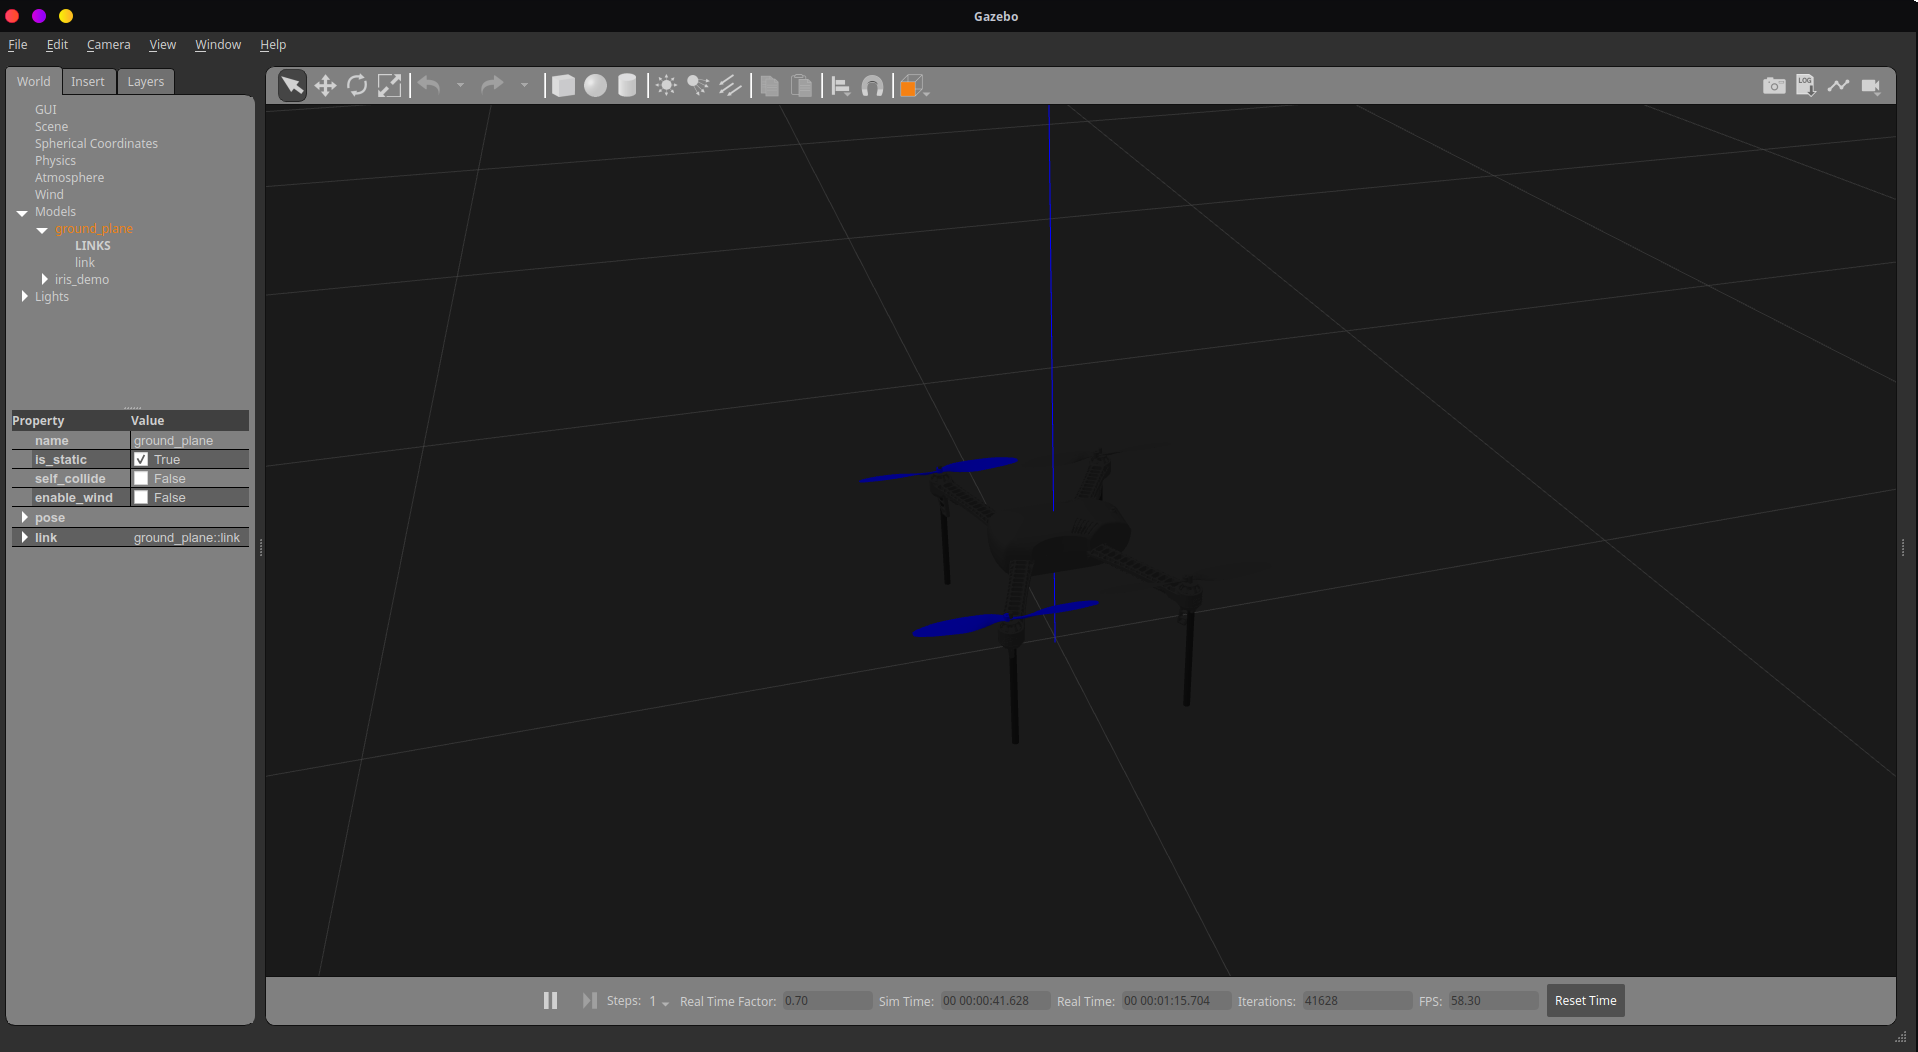
\includegraphics[width=\textwidth]{Gazebo_SITL.png}
    \caption{Modelo en Gazebo del dron Iris}
    \label{fig:Gazebo_SIL}
\end{figure}

\begin{figure}[ht]
    \centering
    \subfloat[Posición inicial]{\label{fig:Ardupilot_sim1}{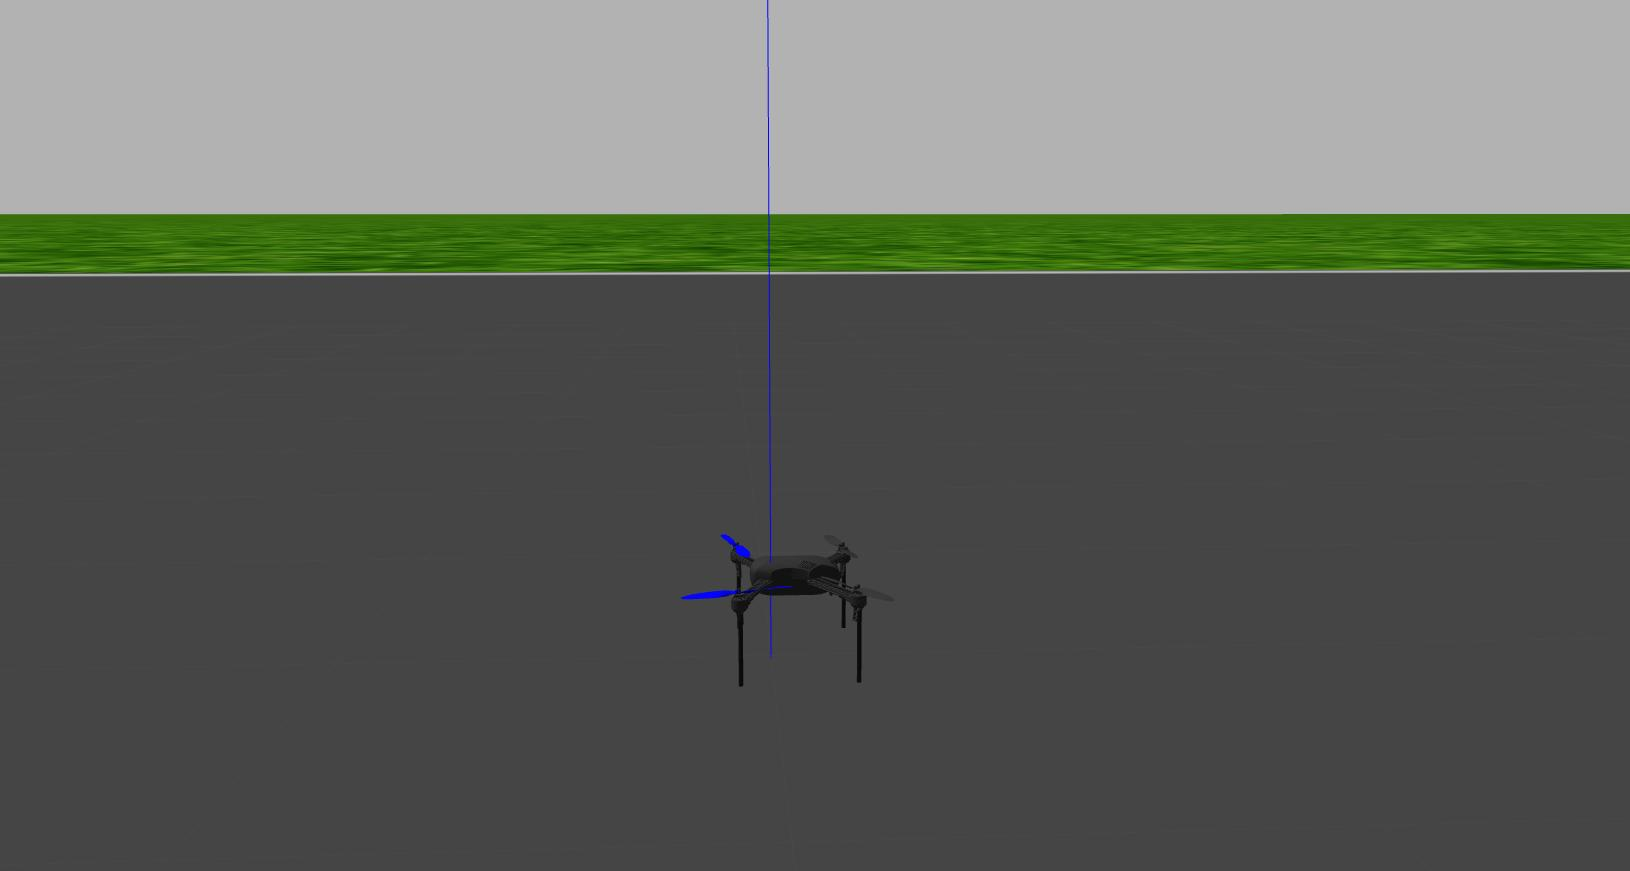
\includegraphics[width=0.48\textwidth]{Ardupilot_sim1.jpg}}}\hfill
    \subfloat[Despegue]{\label{fig:Ardupilot_sim2}{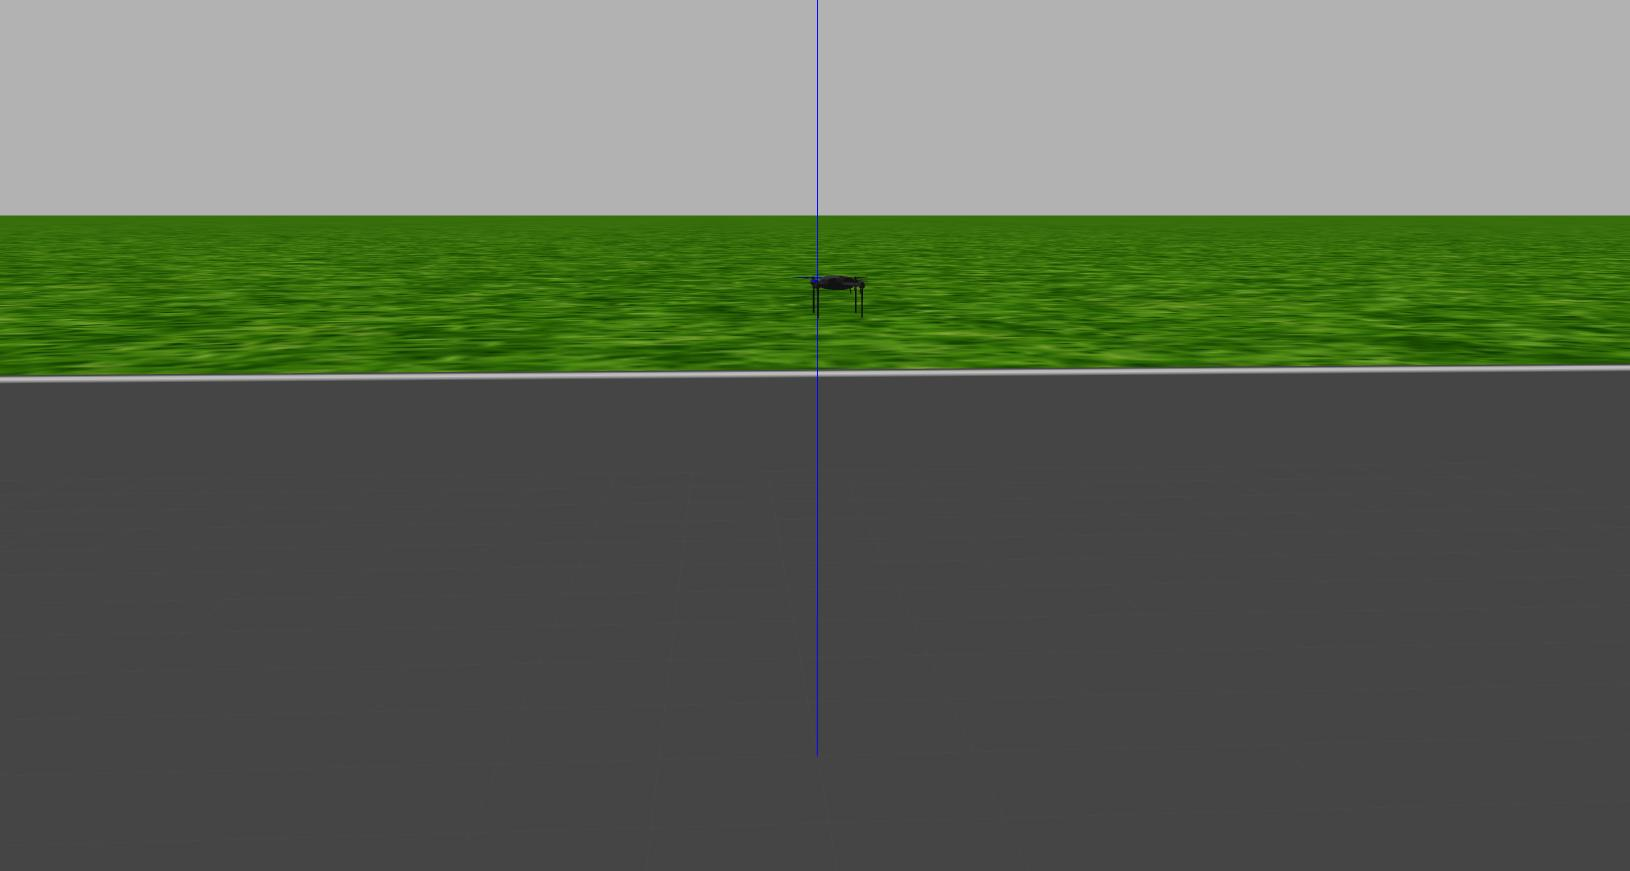
\includegraphics[width=0.48\textwidth]{Ardupilot_sim2.jpg}}}\\
    \subfloat[Movimiento de 20 m en x]{\label{fig:Ardupilot_sim3}{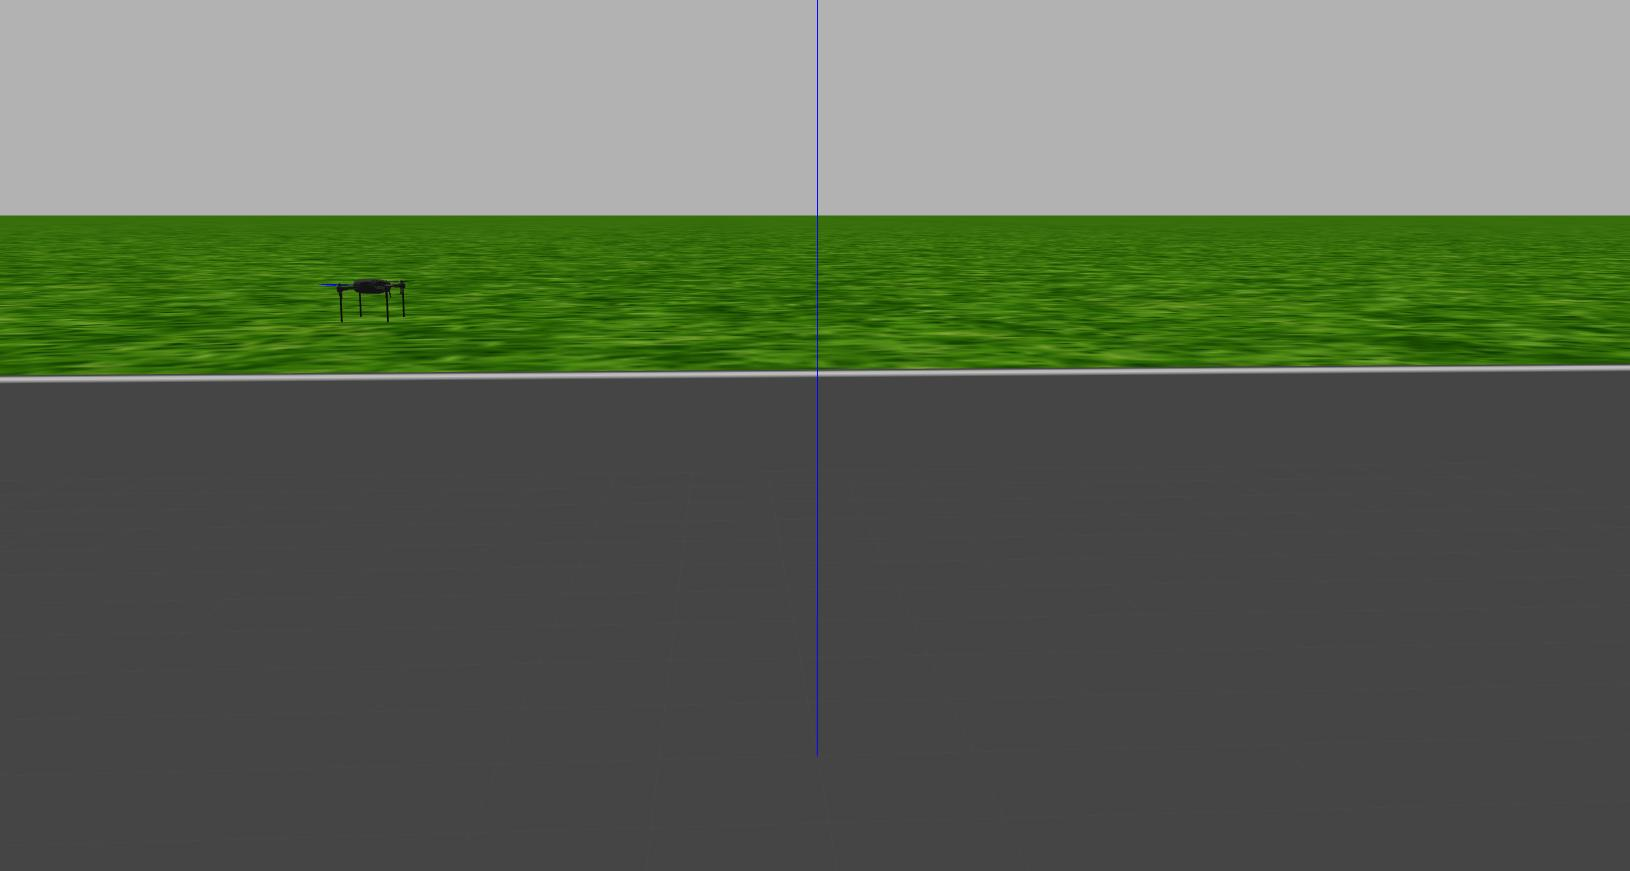
\includegraphics[width=0.48\textwidth]{Ardupilot_sim3.jpg}}}\hfill
    \subfloat[Terminal de ArduPilot lista para recibir comandos de vuelo]{\label{fig:Ardupilot_Ready}{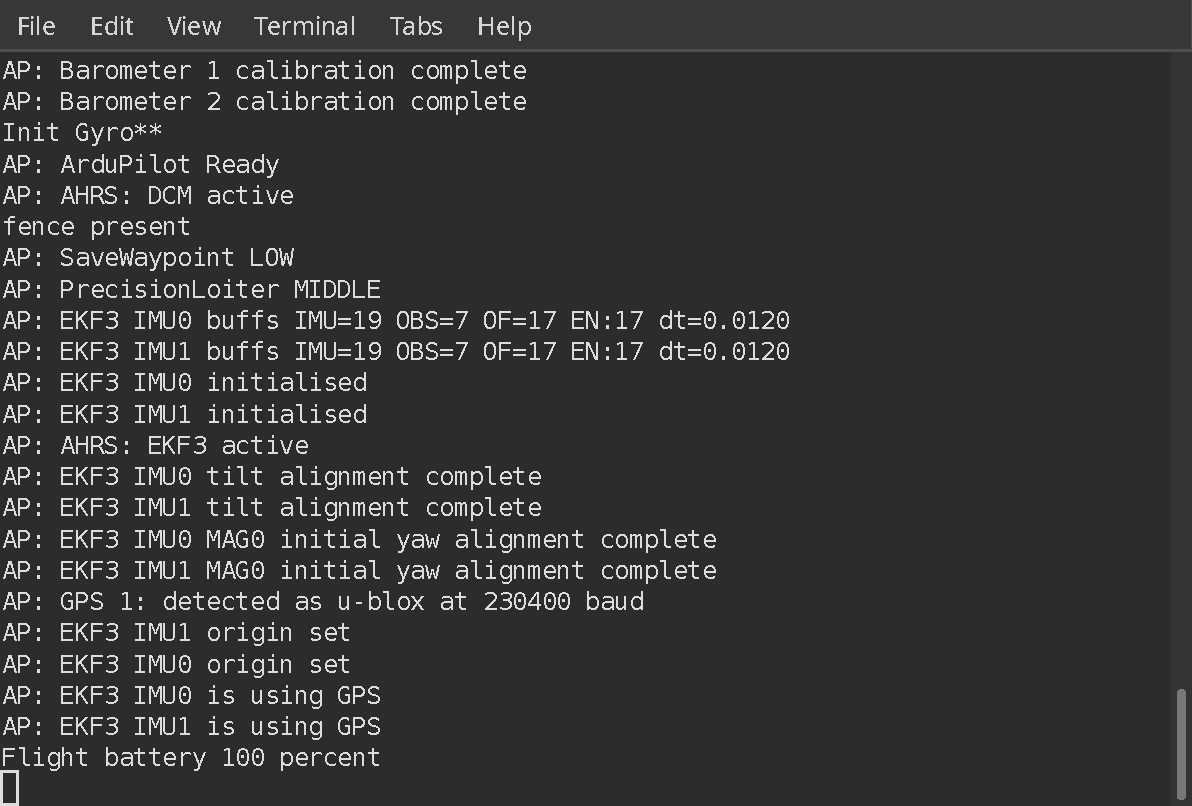
\includegraphics[width=0.48\textwidth]{ArduPilot_Ready.pdf}}}
    \caption{Prueba de integración entre Gazebo y el SIL de ArduPilot}
    \label{fig:Gazebo_Ardupilot}
\end{figure}

\subsection{Instalación de Pymavlink}
Por último, en cuento a la configuración del sistema, es necesario instalar Pymavlink para entablar la comunicación con el framework SIL de ArduPilot, de tal manera que se puedan enviar instrucciones de modos de vuelo, así como comandos que permitan definir la trayectoria de vuelo del dron, a través de un script en Python sin necesidad de ingresar estas instrucciones directamente en una terminal.

La librería Pymavlink está contenida en un módulo de Python, por lo que su instalación resulta un tanto trivial; sin embargo, cabe destacar que es necesario haber instalado el gestor de paquetes de Python 3 para ejecutar los siguientes comandos:

\begin{enumerate}
    \item Actualizar los repositorios y paqueterías del sistema
    \begin{lstlisting}[language = bash]
        $ sudo apt update && sudo apt -y full-upgrade
    \end{lstlisting} 
    
    \item Instala el módulo que contiene la librería
    \begin{lstlisting}[language = bash]
        $ pip3 install mavproxy
    \end{lstlisting} 
\end{enumerate}

Para verificar la instalación de la librería se puede abrir el intérprete de Python 3 en una terminal y transcribir la siguiente serie de comandos

\begin{lstlisting}[language = bash]
    $ python3
    >>> import pymavlink
    >>> print(pymavlink.__doc__)
\end{lstlisting} 

Al ejecutar lo anterior, se debe de generar una impresión en la terminal de la figura \ref{fig:Pymavlink_ver}.

\begin{figure}[ht]
    \centering
    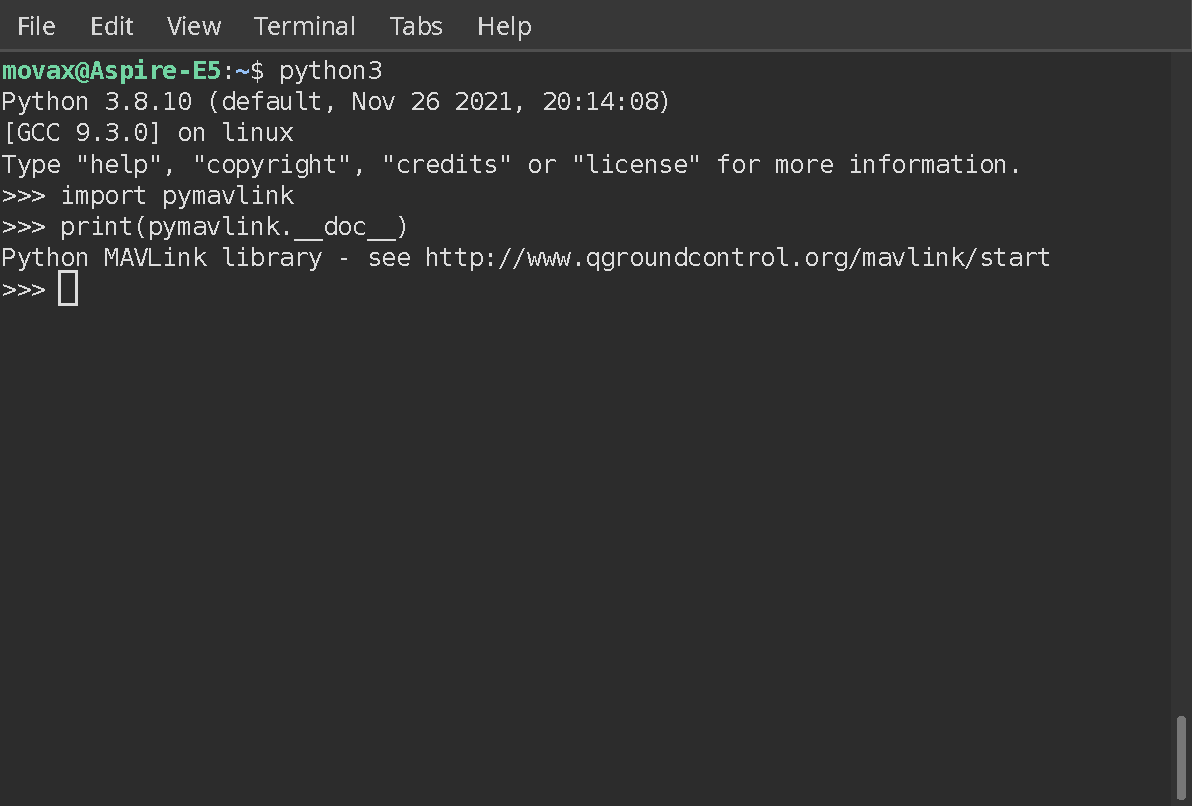
\includegraphics[width=0.7\textwidth]{Pymavlink_ver.pdf}
    \caption{Validación de instalación de Pymavlink}
    \label{fig:Pymavlink_ver}
\end{figure}


\section{Circuito de Vuelo Virtual}
La sección anterior corresponde a la configuración que se realizó para instalar y validar las herramientas que se utilizaron para la elaboración del proyecto. En los siguientes capítulos se detallan el uso específico que se le dio al software instalado, así como las pruebas y los resultados obtenidos; en esta sección se especifica el proceso de elaboración de la simulación con el circuito de vuelo para el dron simulado.

La figura \ref{fig:Circuit} presenta un diagrama con en donde se especifica la estructura del circuito elaborado, en él se pueden apreciar las cotas con las distancias presentes entre cada una de las compuertas, así como el orden del recorrido realizado por el dron. Cabe destacar que el modelo de compuerta que se seleccionó para el circuito de vuelo, fue el utilizado en las distintas competencias del IROS.

\begin{figure}[ht]
    \centering
    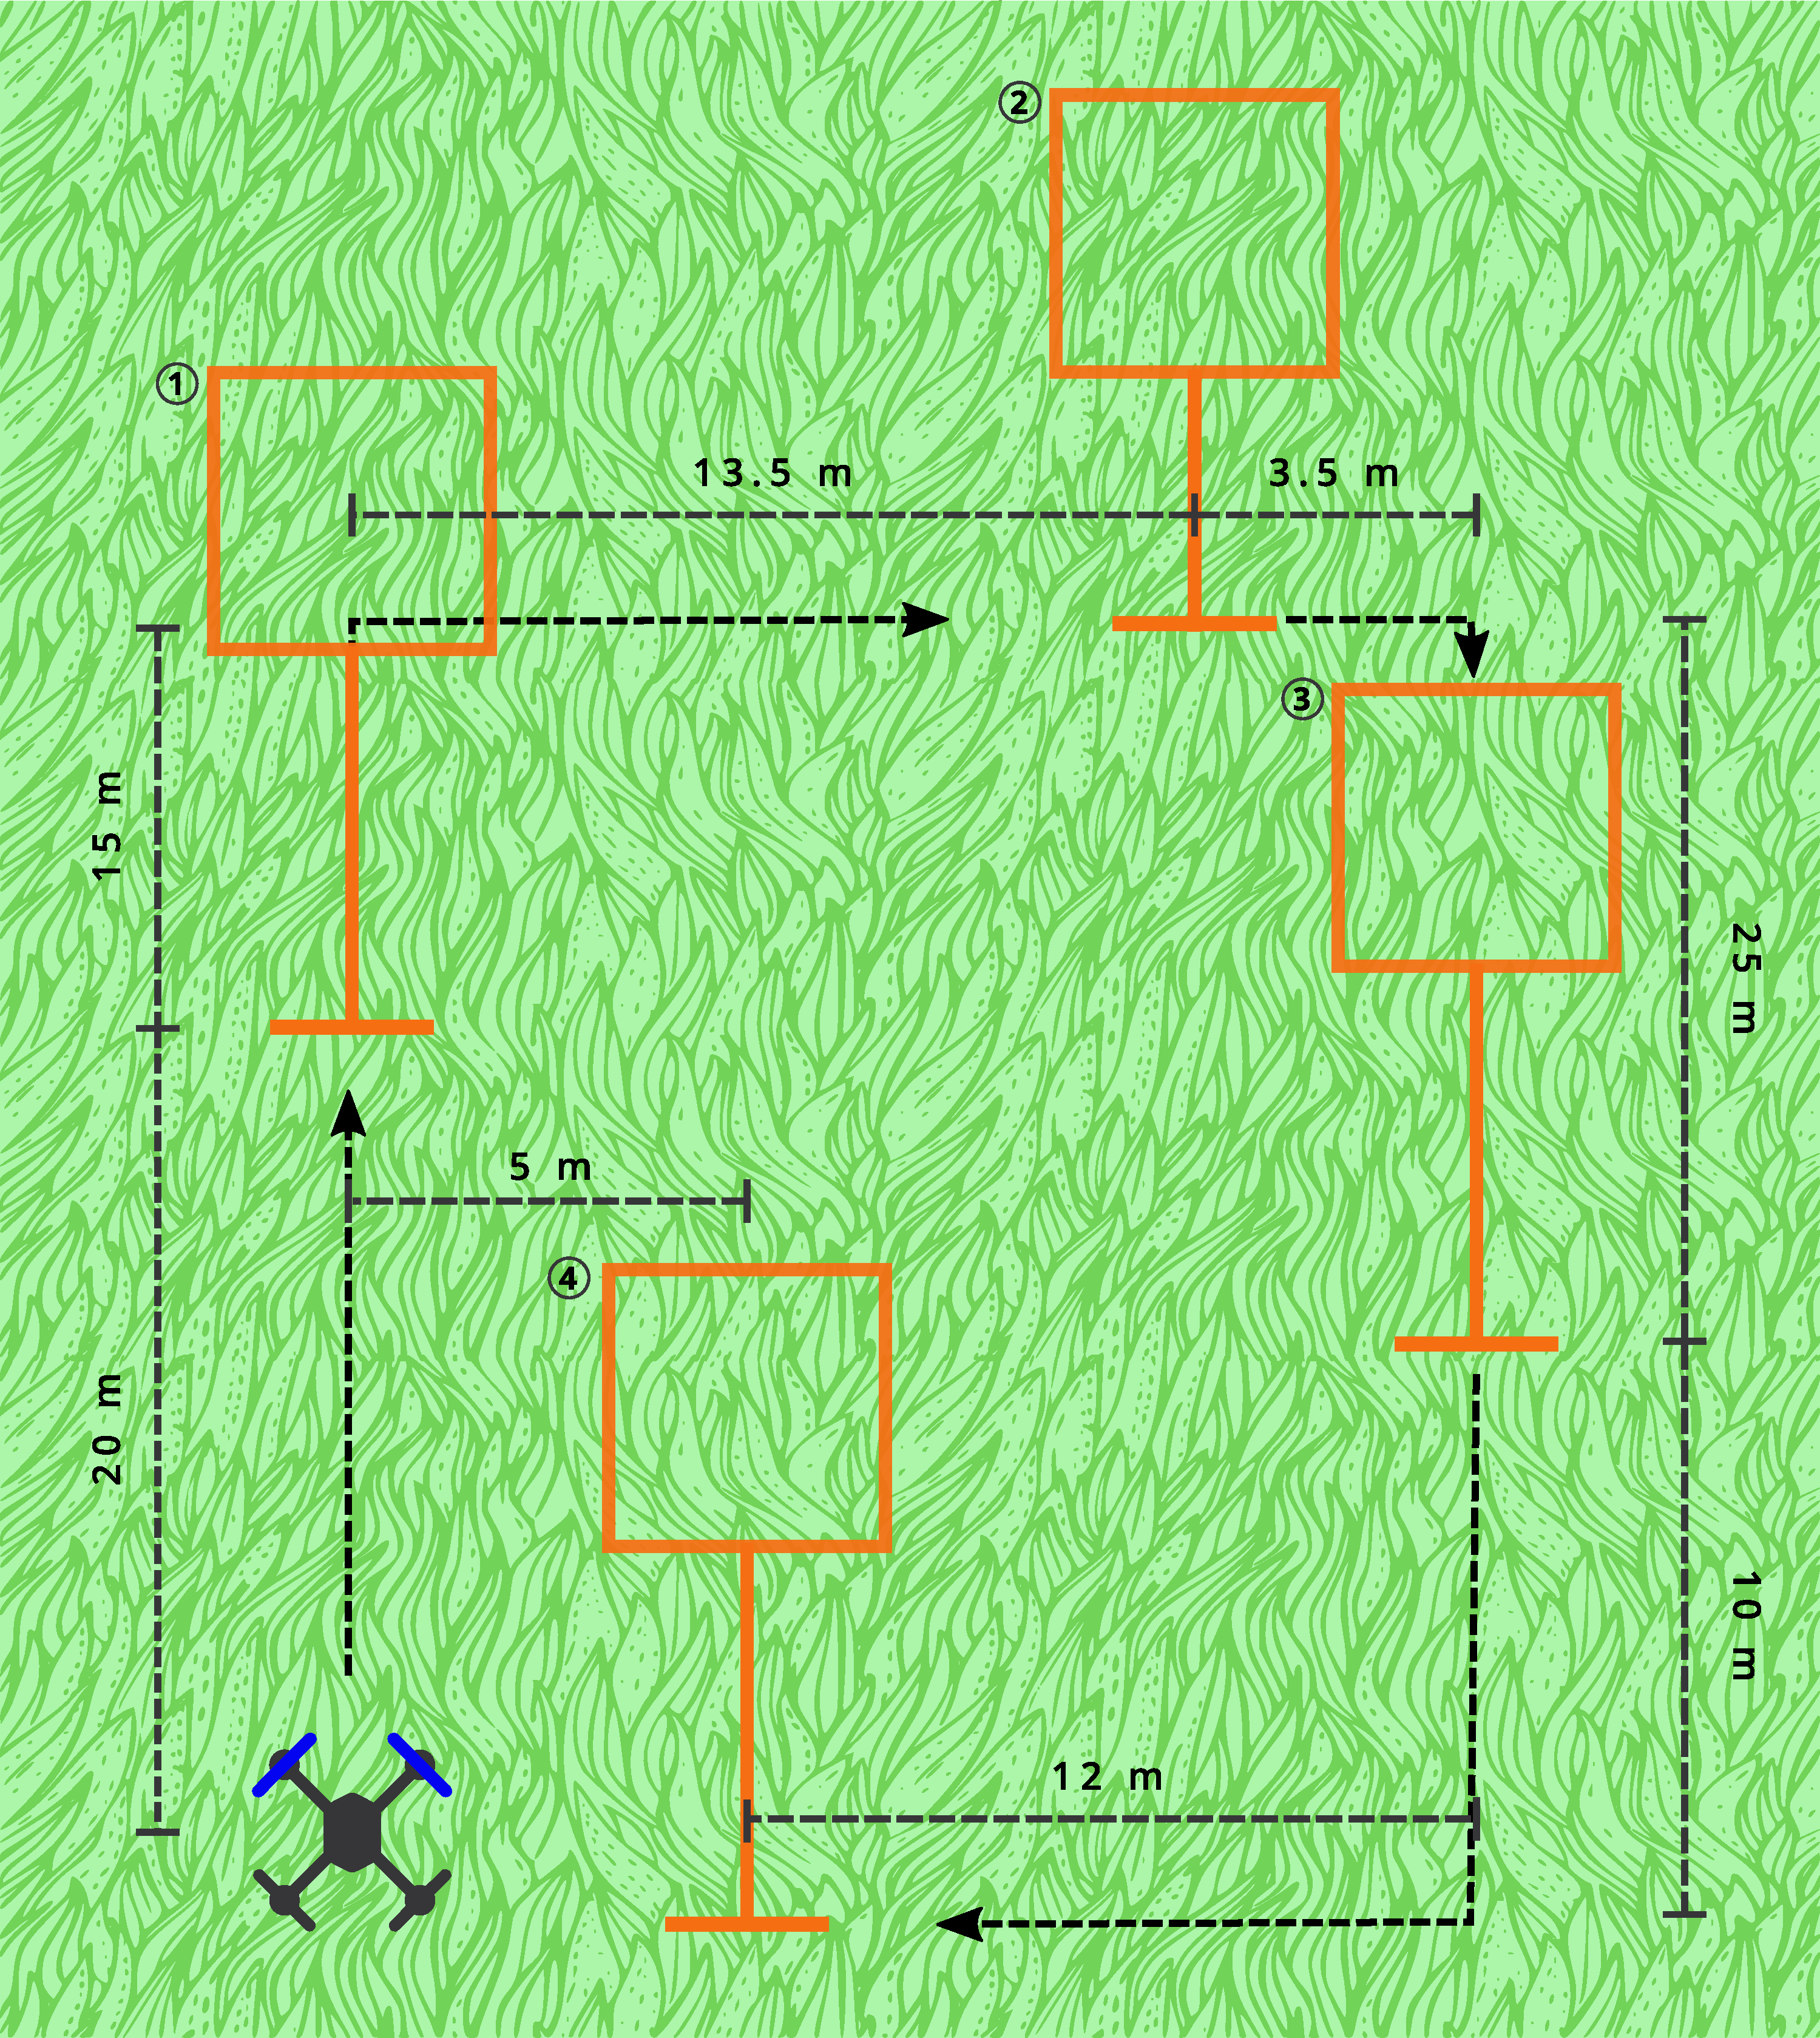
\includegraphics[width=0.8\textwidth]{Circuit.pdf}
    \caption{Esquema detallado del circuito de vuelo elaborado en simulación.}
    \label{fig:Circuit}
\end{figure}

A partir del esquema antes mencionado, la elaboración del circuito dentro de la simulación se llevó a cabo utilizando algunos modelos ya elaborados por la comunidad de Gazebo. Para el terreno y el modelo de la compuerta se utilizaron los modelos elaborados por \cite{rojas2020deeppilot}, los cuales fueron usados para entrenar su red neuronal profunda. Por otro lado, el modelo del dron Iris fue provisto por

Por otro lado, existe un bug al utilizar Gazebo, pues al crear mundo nuevo, no es posible guarda el proyecto con los cambios realizados, el menú de diálogo que aparece la opción de guarda proyecto simplemente no se muestra de forma correcta, por lo que crear un proyecto nuevo resulta imposible de esta forma. Debido o a lo anterior, en este trabajo se propone una solución para sobrellevar el problema anterior; para que el menú se muestre de forma correcta es necesario ejecutar Gazebo con permisos de administrador; sin embargo, al utilizar privilegios de administrador para crear el archivo del proyecto, este se encontrará protegido contra escritura, y resulta muy poco práctico necesitar permisos de administrador para realizar modificaciones sobre el proyecto.

Entonces, para solucionar este segundo problema se debe de crear un archivo utilizando el comando \textit{touch} con la extensión \textit{.world}. Lo anterior genera un archivo un proyecto de Gazebo completamente vacío. Ahora, debido a que este tipo de archivos solamente contiene la descripción de los componentes utilizados en determinado proyecto, así como sus características físicas como posición, es posible abrir el archivo del proyecto con cualquier editor de texto y ver su contenido. Por lo tanto, se puede copiar el contenido del proyecto creado con privilegios de administrador y pegarlo dentro del nuevo proyecto vacío que se acaba de crear.

Hecho lo anterior, lo que queda es eliminar el proyecto protegido contra escritura. Para ello es necesario abrir una terminal dentro del directorio donde se encuentra el proyecto y ejecutar el comando \textit{rm} con permisos de administrador. A continuación se anexa un ejemplo:

\begin{lstlisting}[language = bash]
    $ sudo rm proyectName.world
\end{lstlisting} 

La figura \ref{fig:Gazebo_gates} muestra los modelos 3D utilizados para la elaboración de la simulación; como se mencionó, se ocuparon dos tamaños de compuerta y por lo tanto dos modelos.

Adicionalmente, la figura \ref{fig:Gazebo_iris} presenta el modelo 3D del dron iris utilizado. Cabe destacar que la principal diferencia entre el modelo provisto por \cite{IQ} y el modelo incluido en la simulación de demostración del plugin de Ardupilot para Gazebo, es la orientación de la cámara. En la simulación de demostración, la cámara se encuentra apuntando hacia el suelo, mientras que en el modelo mostrado en la figura, apunta hacía al frente de la dirección de vuelo del dron.

\begin{figure}[ht]
    \centering
    \subfloat[Vista frontal del modelo de compuerta grande]{\label{fig:Gazebo_gate1}{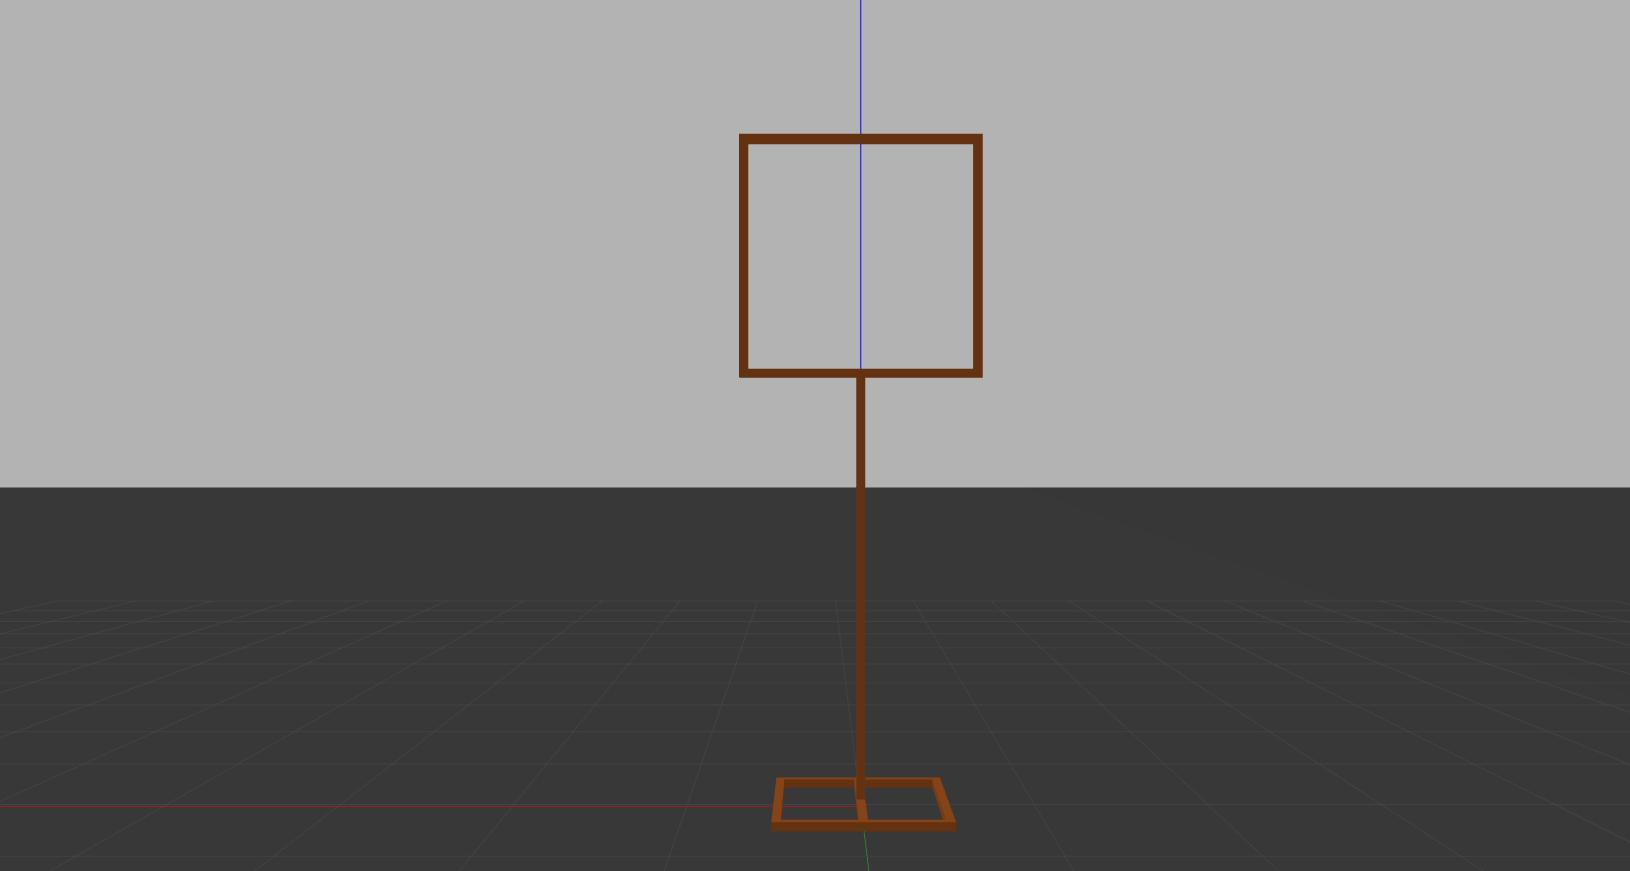
\includegraphics[width=0.48\textwidth]{Gazebo_gate1.jpg}}}\hfill
    \subfloat[Vista superior del modelo de compuerta grande]{\label{fig:Gazebo_gate2}{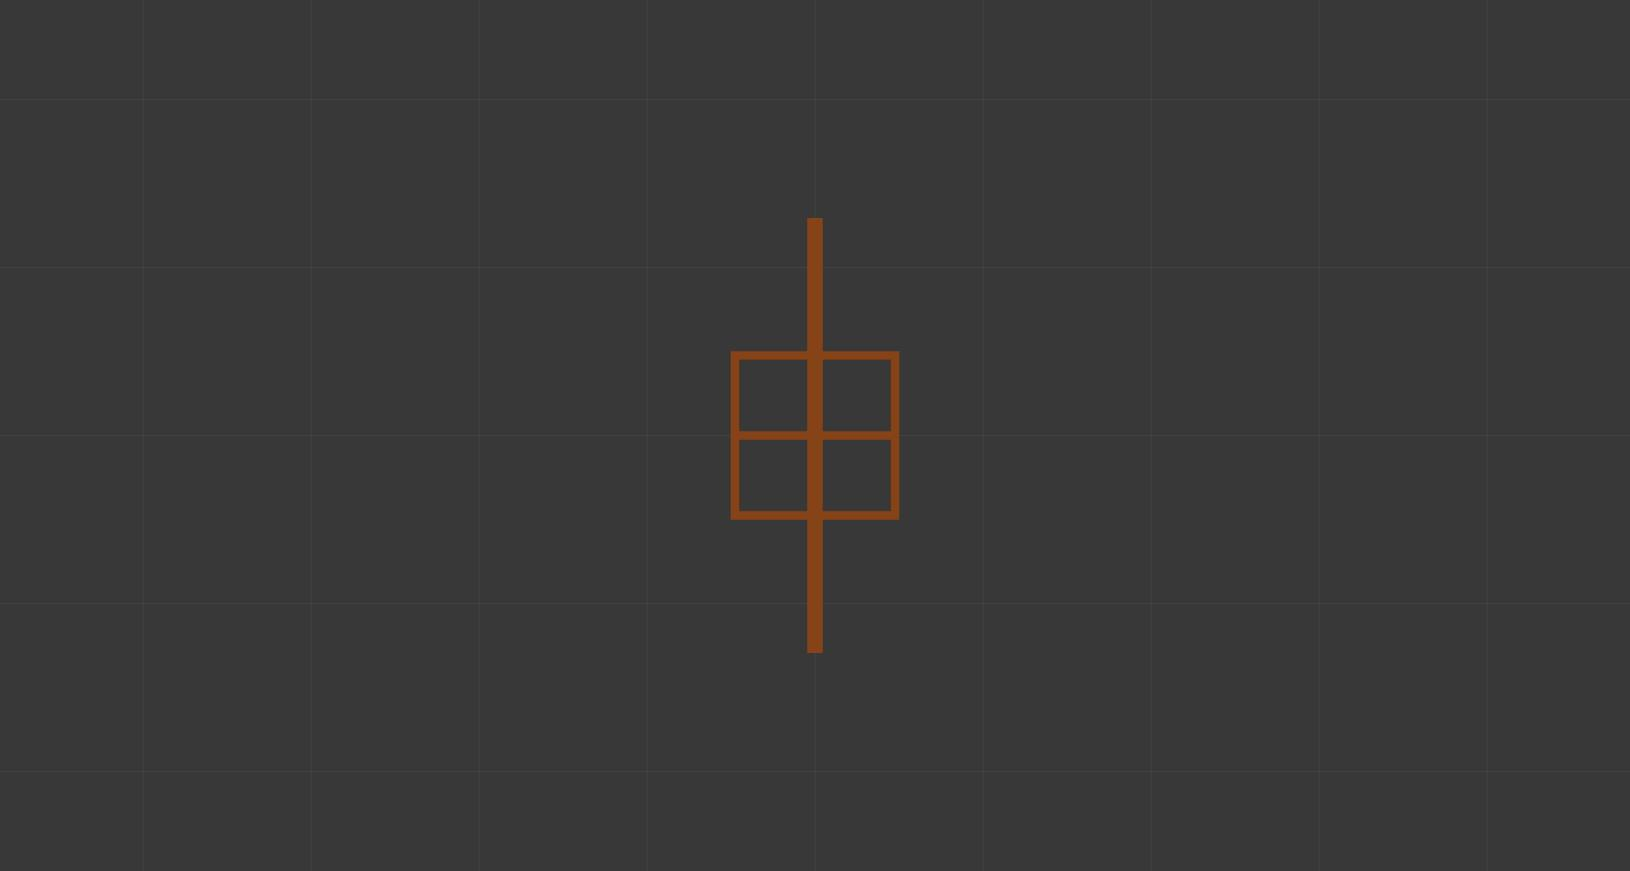
\includegraphics[width=0.48\textwidth]{Gazebo_gate2.jpg}}}\\
    \subfloat[Vista frontal del modelo de compuerta mediana]{\label{fig:Gazebo_gate3}{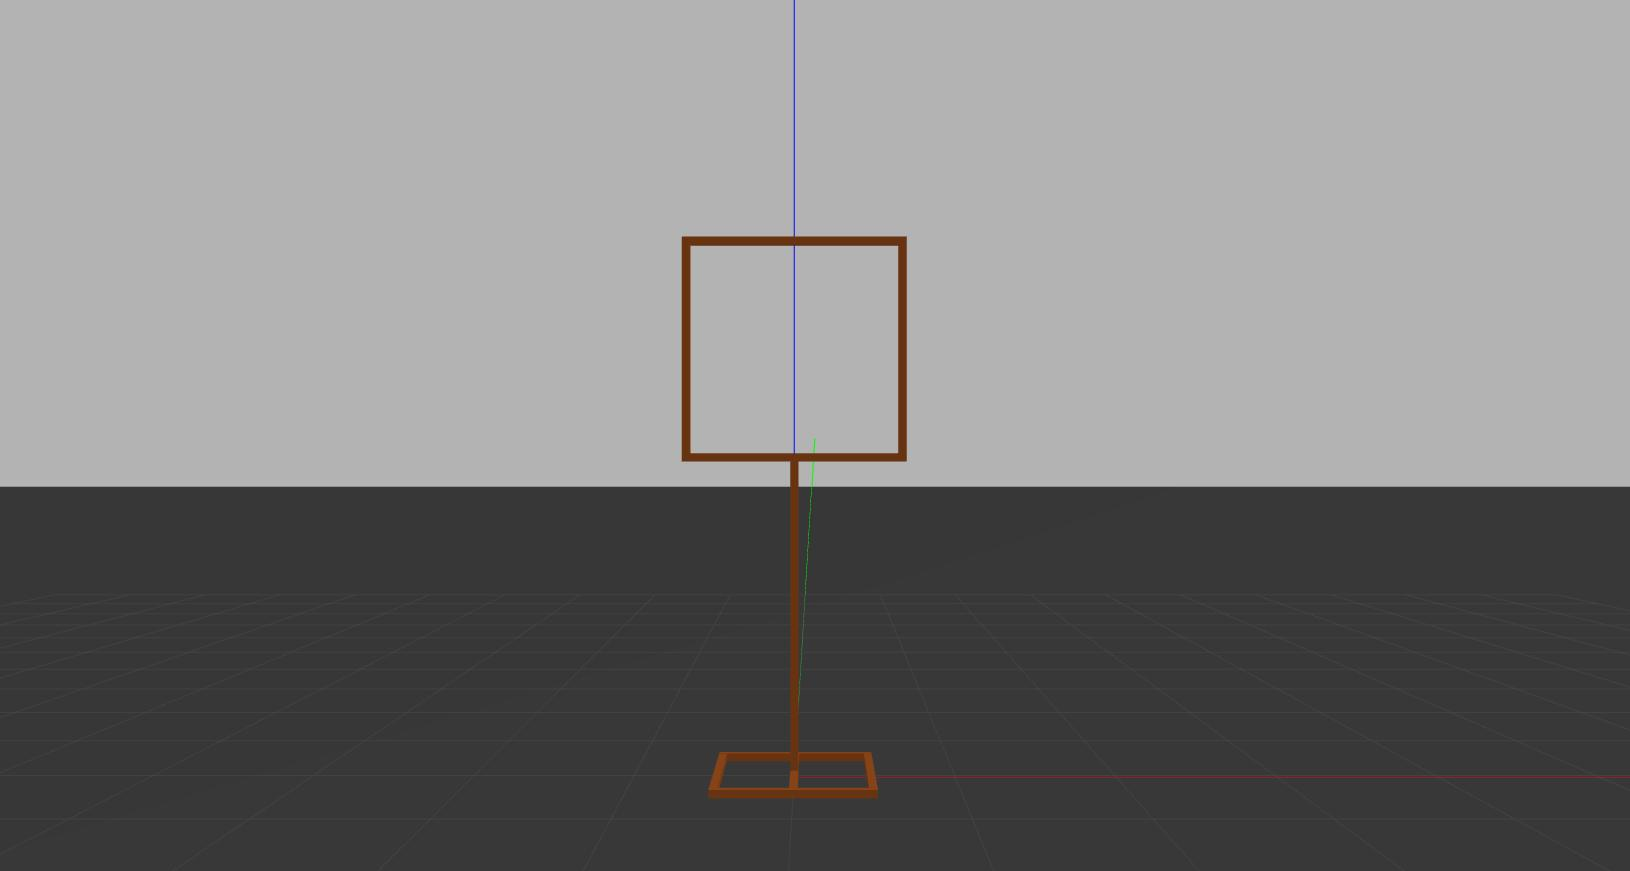
\includegraphics[width=0.48\textwidth]{Gazebo_gate3.jpg}}}\hfill
    \subfloat[Vista superior del modelo de compuerta mediana]{\label{fig:Gazebo_gate4}{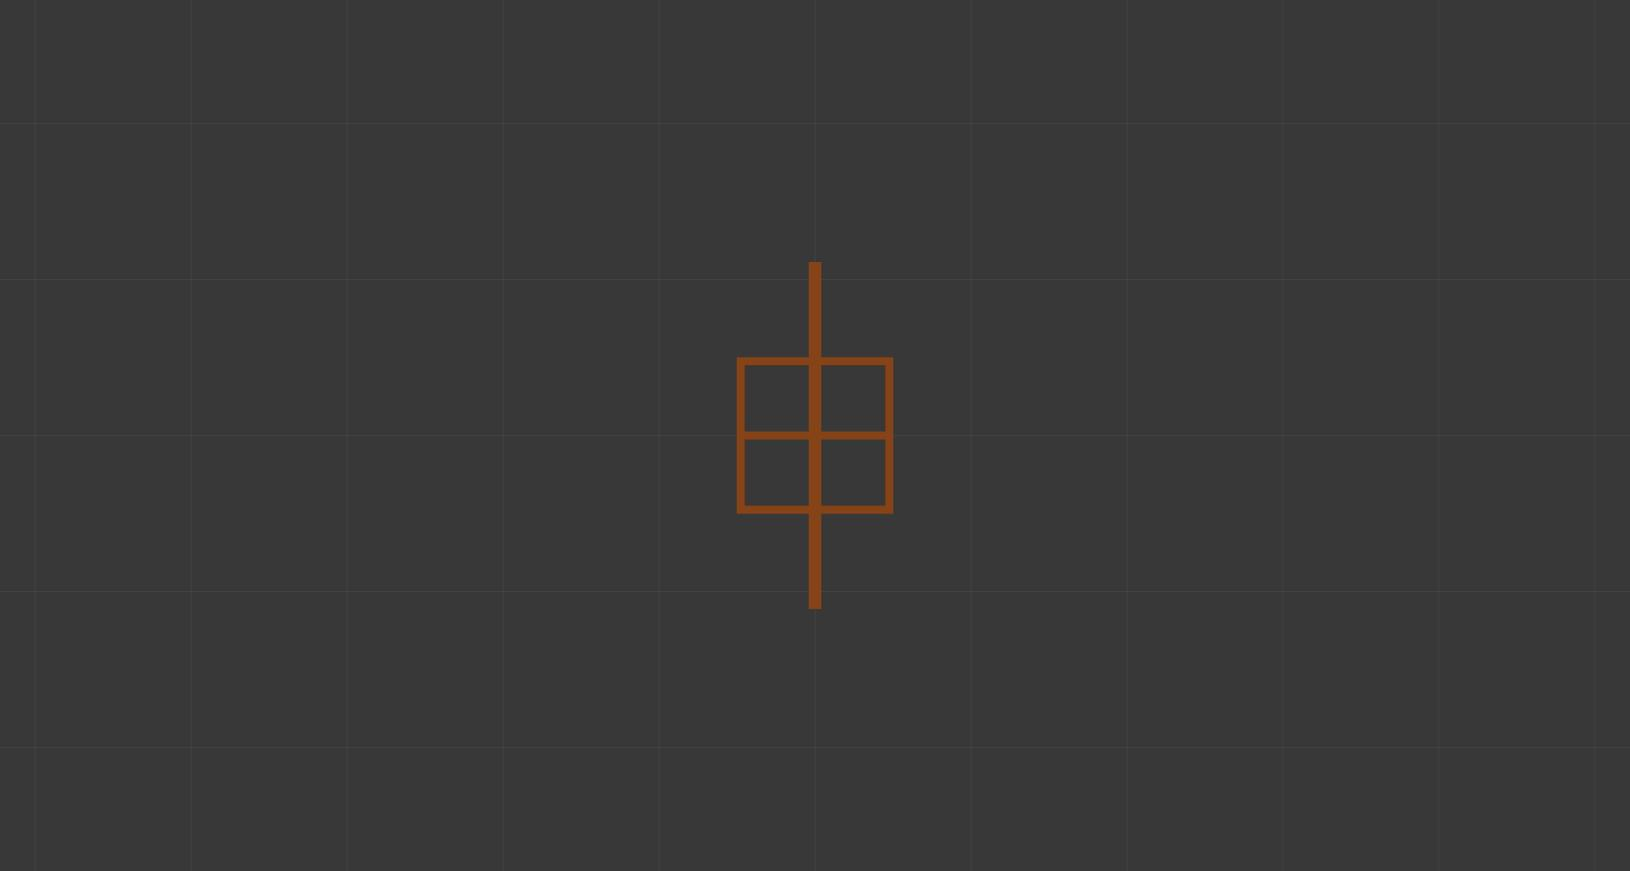
\includegraphics[width=0.48\textwidth]{Gazebo_gate4.jpg}}}
    \caption{Modelos de compuerta proveídos por \cite{rojas2020deeppilot}}
    \label{fig:Gazebo_gates}
\end{figure}

\begin{figure}[ht]
    \centering
    \subfloat[Vista trasera]{\label{fig:Gazebo_iris1}{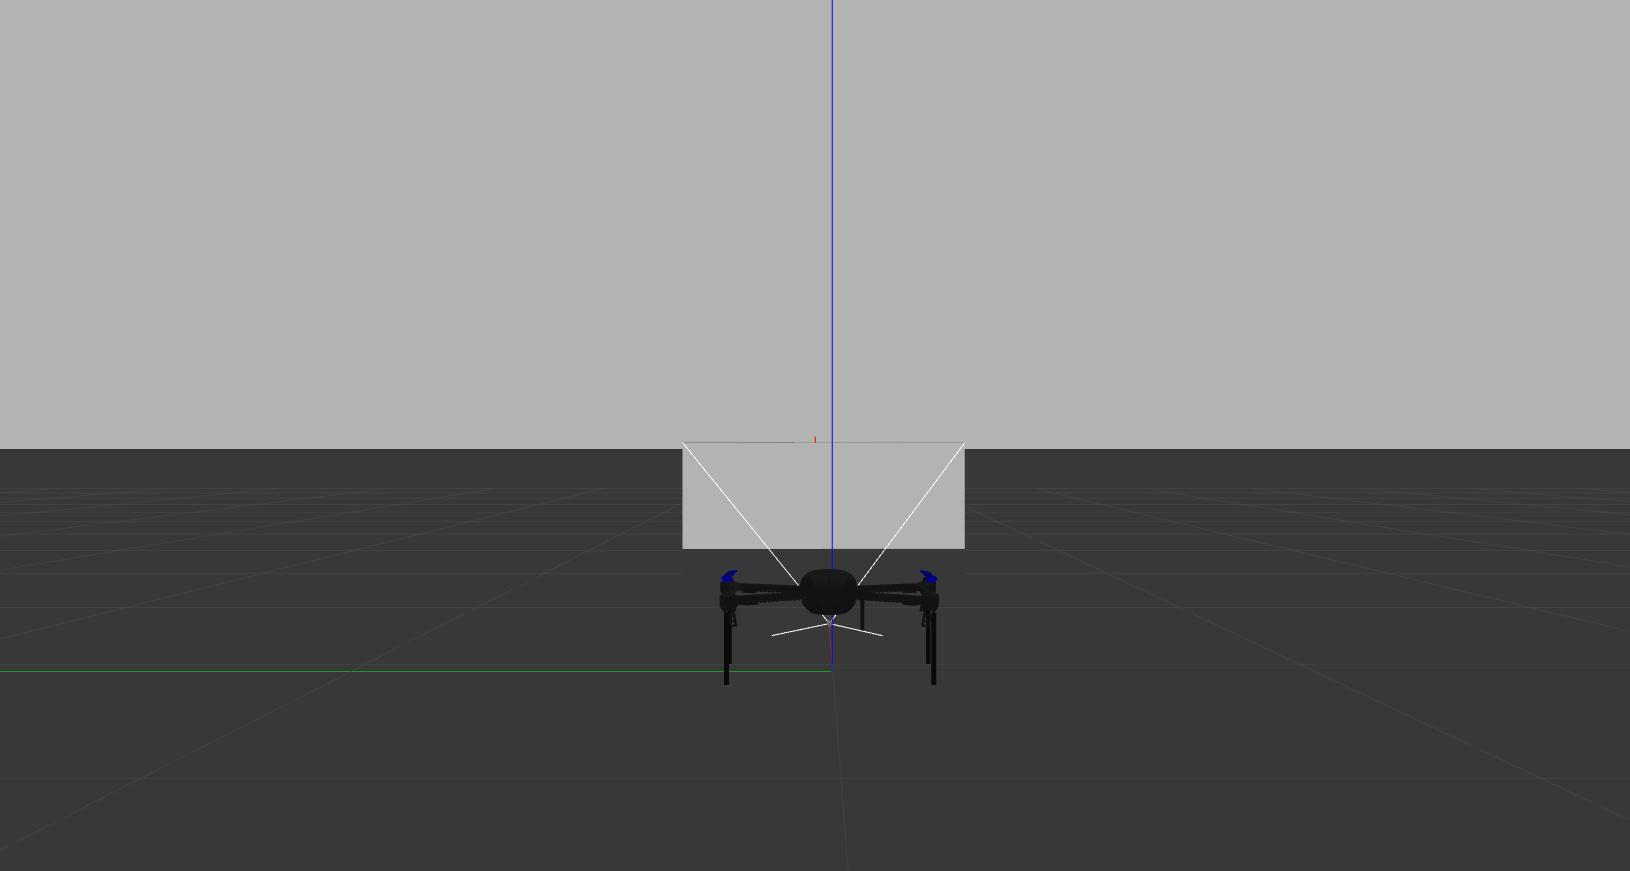
\includegraphics[width=0.48\textwidth]{Gazebo_iris1.jpg}}}\hfill
    \subfloat[Vista lateral]{\label{fig:Gazebo_iris2}{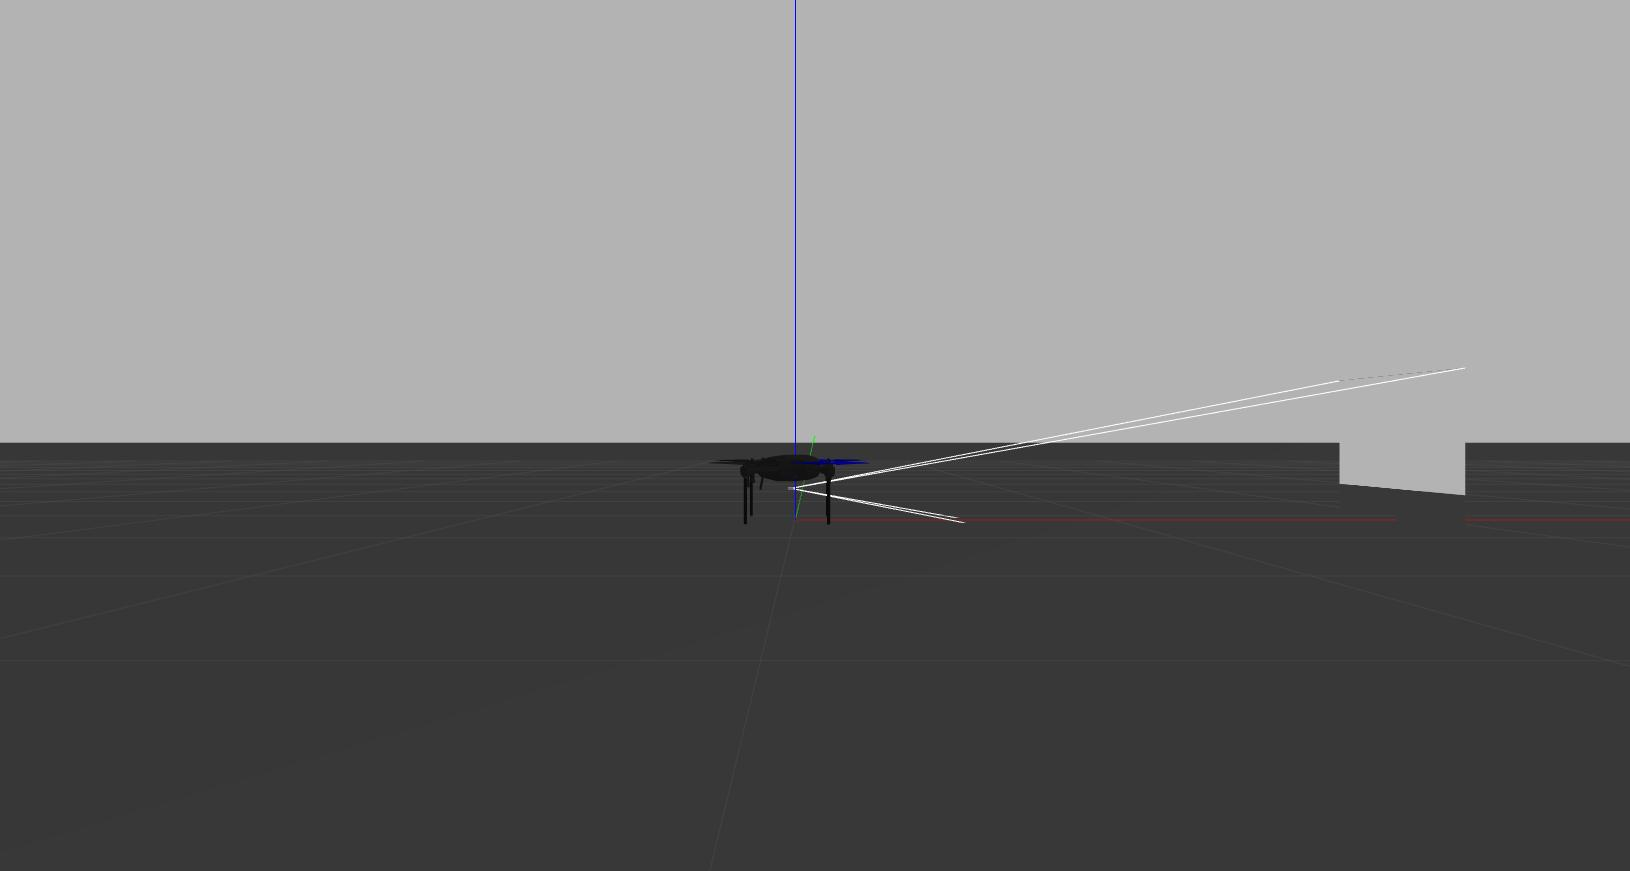
\includegraphics[width=0.48\textwidth]{Gazebo_iris2.jpg}}}\\
    \subfloat[Vista superior]{\label{fig:Gazebo_iris3}{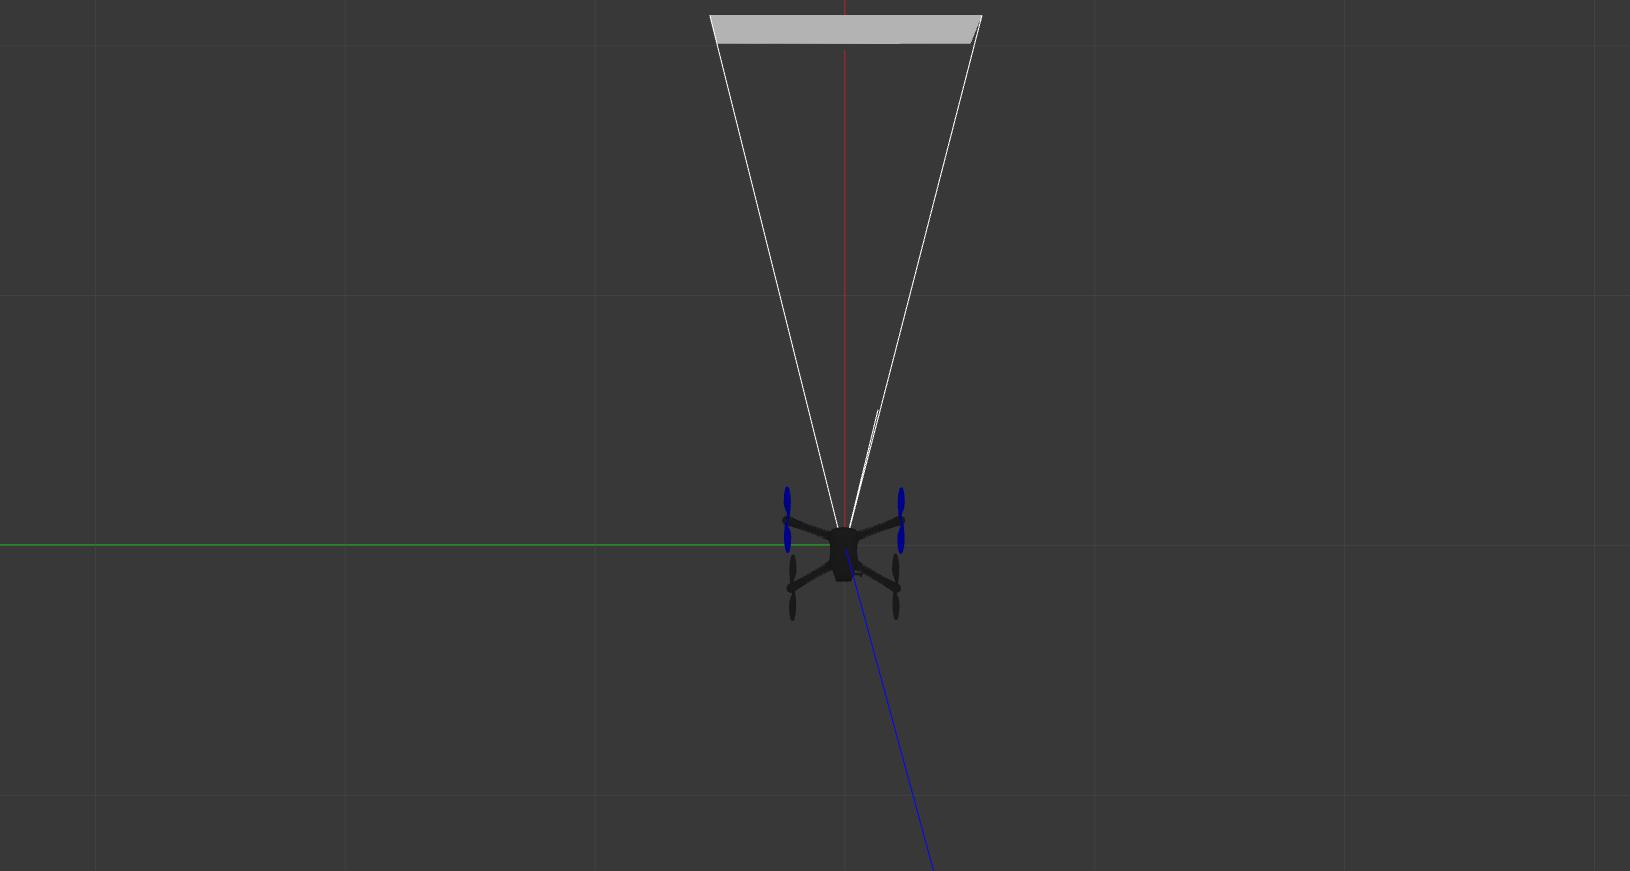
\includegraphics[width=0.48\textwidth]{Gazebo_iris3.jpg}}}\hfill

    \caption{Modelo de dron iris con cámara frontal provisto por \citet{IQ}}
    \label{fig:Gazebo_iris}
\end{figure}


Por último, la figura \ref{fig:Gazebo_worlds} muestra algunas capturas tomadas dentro del proyecto creado para implementar el circuito de vuelo implementado. La figura \ref{fig:Gazebo_world1} presenta un panorama general del circuito de vuelo, en ella se observan las cuatro compuertas del circuito, el dron iris y el modelo de un edificio; este último se incluyó para fines del algoritmo de visión artificial. Por otro lado, las figura \ref{fig:Gazebo_world2} y \ref{fig:Gazebo_world3}  muestran otras perspectivas del circuito y de los objetos que lo componen. Finalmente, la figura \ref{fig:Gazebo_world4} muestra la perspectiva del dron Iris junto con la toma captada por la cámara simulada en este.

\begin{figure}[ht]
    \centering
    \subfloat[]{\label{fig:Gazebo_world1}{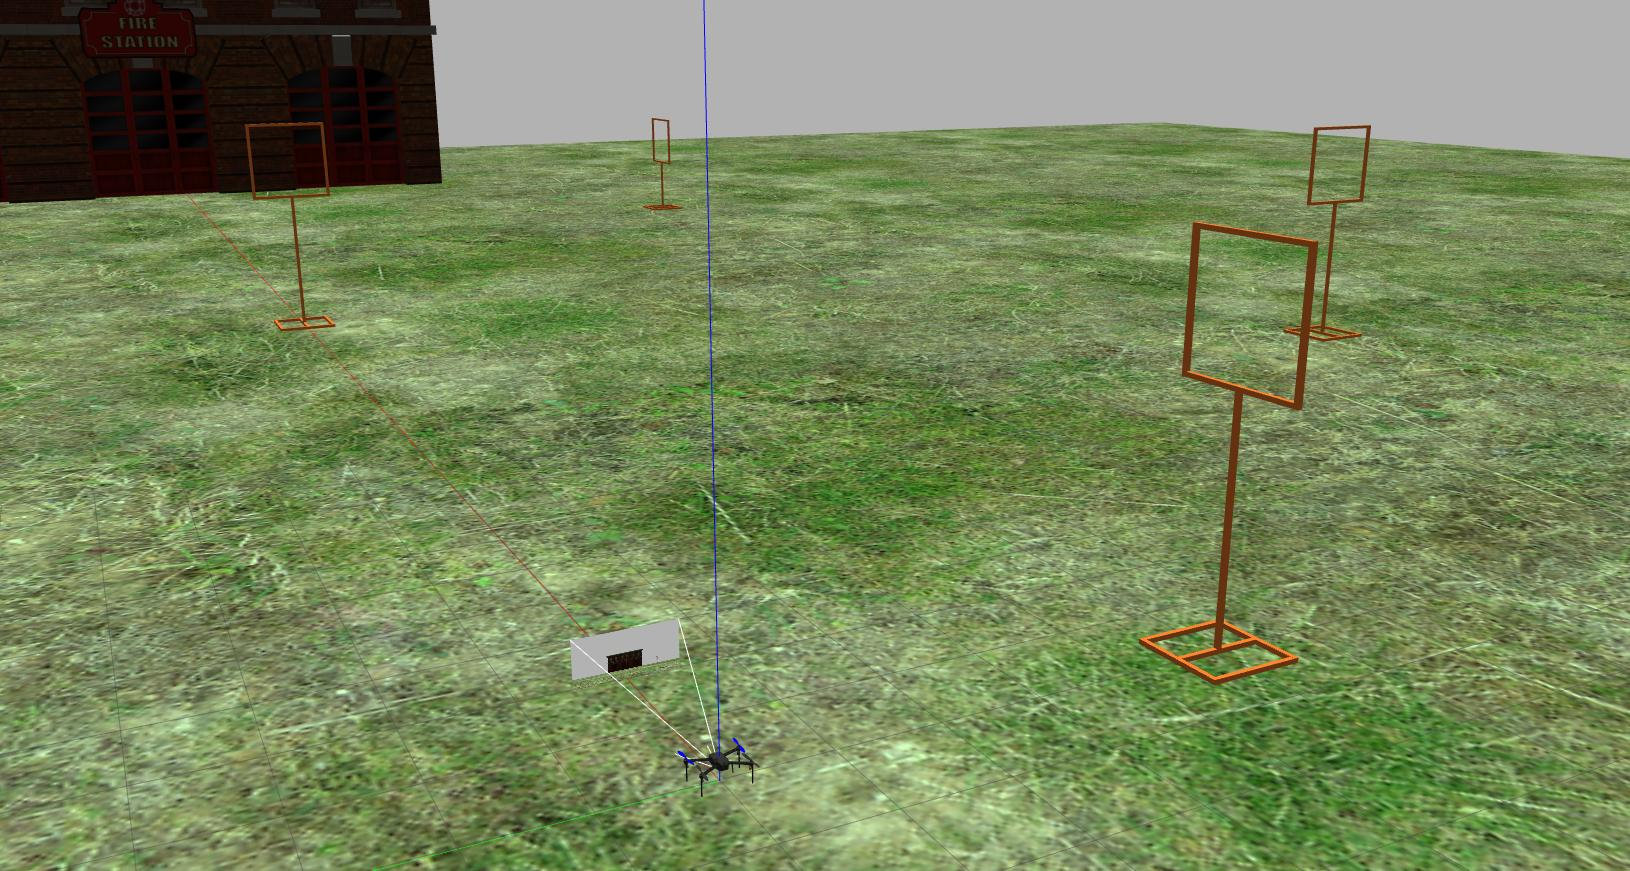
\includegraphics[width=0.48\textwidth]{Gazebo_world1.jpg}}}\hfill
    \subfloat[]{\label{fig:Gazebo_world2}{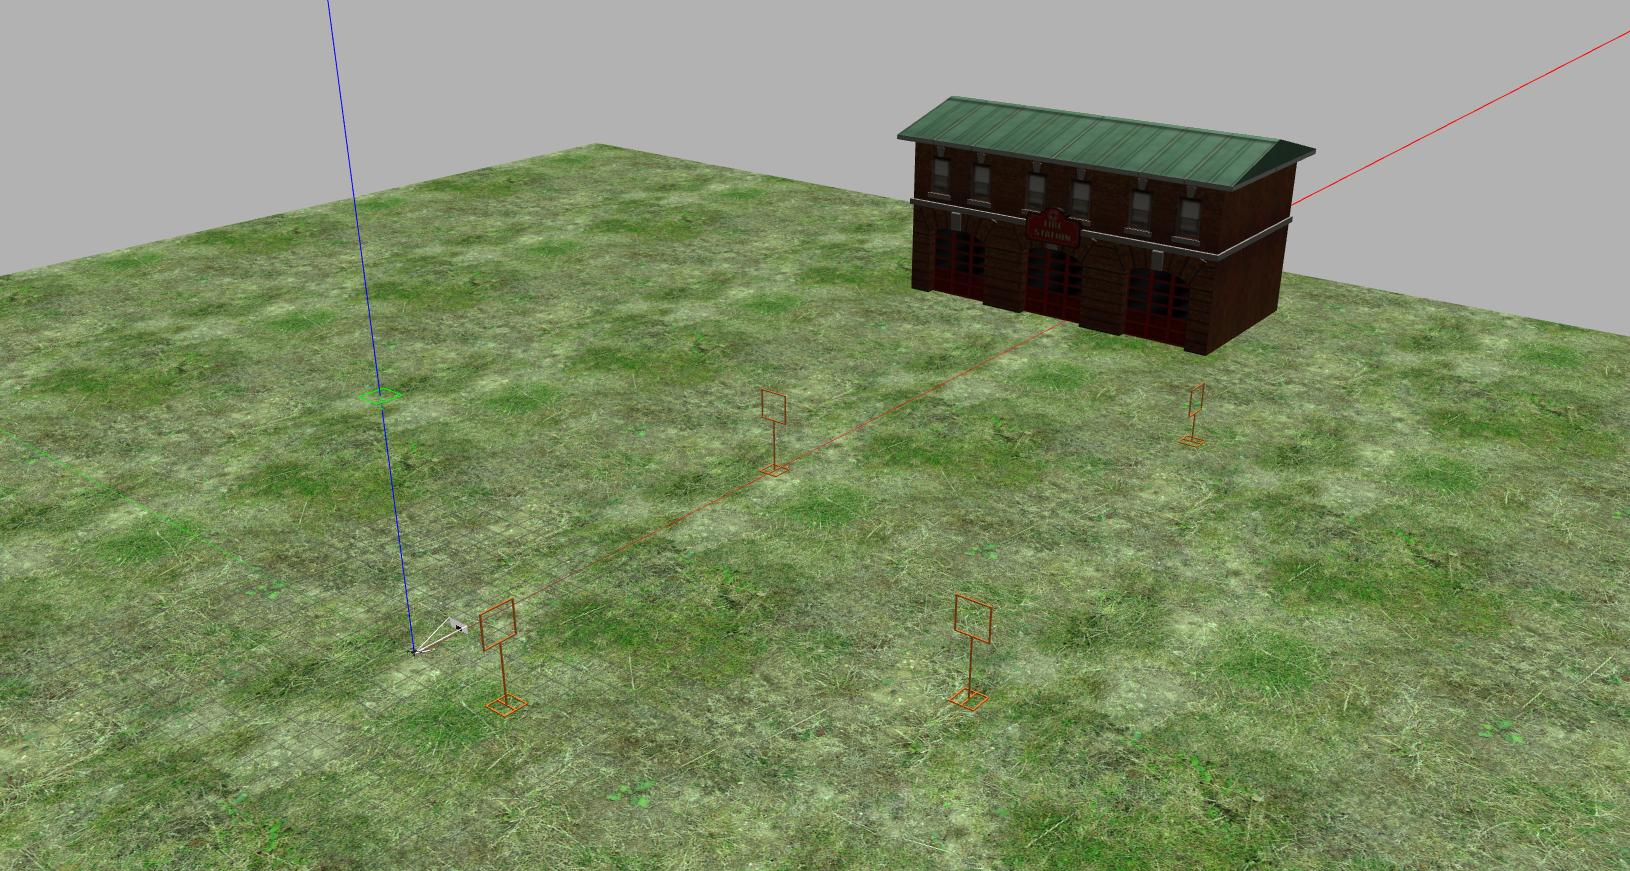
\includegraphics[width=0.48\textwidth]{Gazebo_world2.jpg}}}\\
    \subfloat[]{\label{fig:Gazebo_world3}{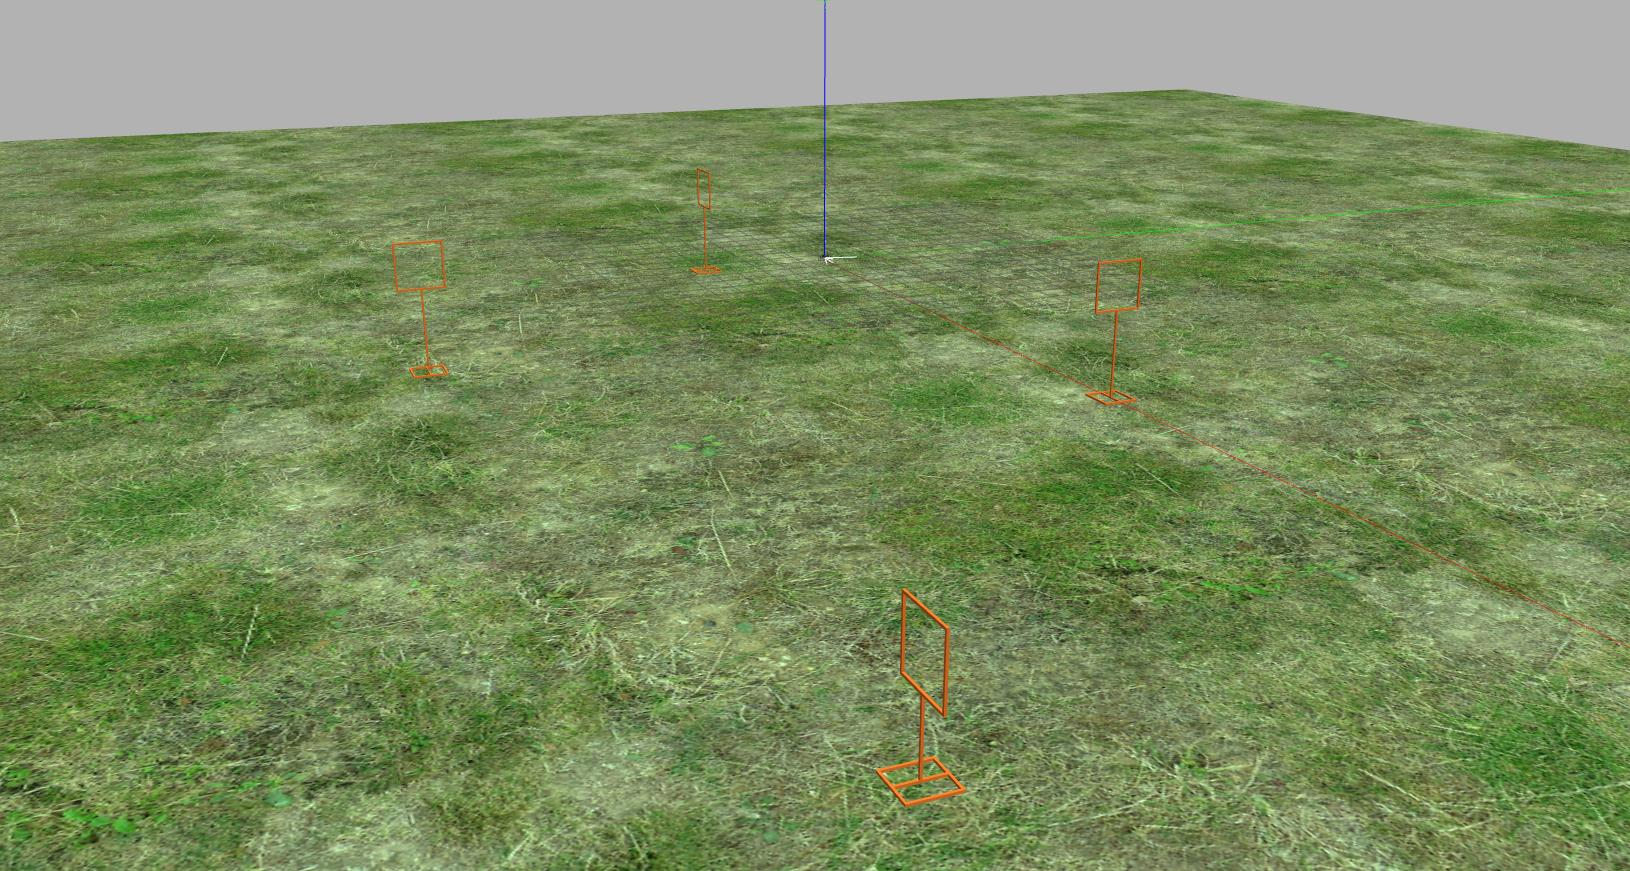
\includegraphics[width=0.48\textwidth]{Gazebo_world3.jpg}}}\hfill
    \subfloat[]{\label{fig:Gazebo_world4}{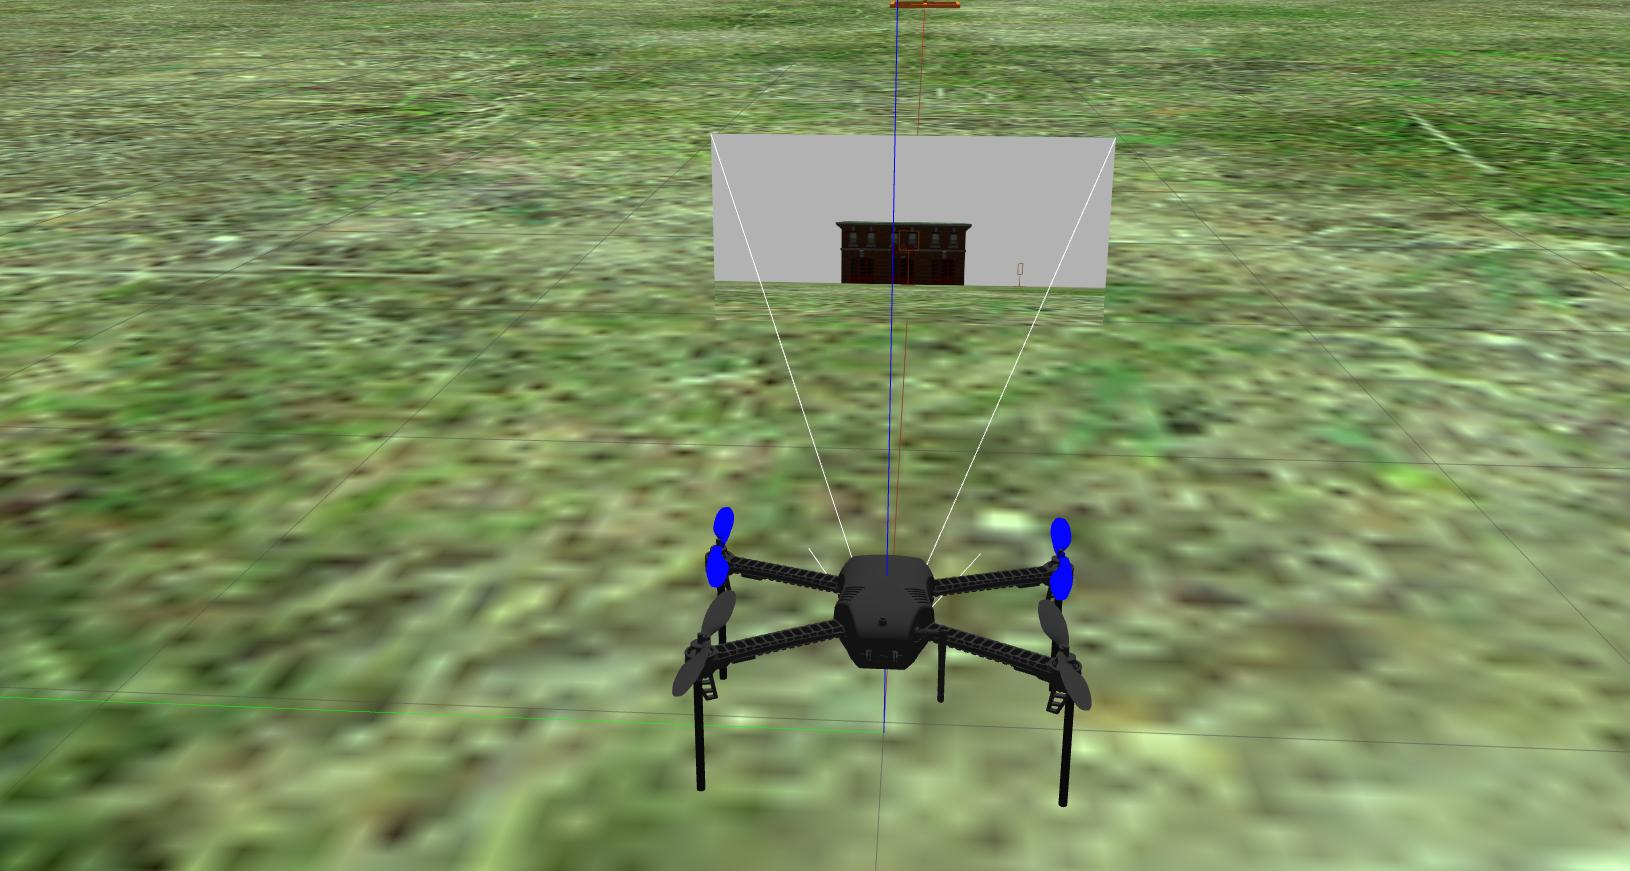
\includegraphics[width=0.48\textwidth]{Gazebo_world4.jpg}}}\hfill

    \caption{Capturas del ambiente de simulación implementado}
    \label{fig:Gazebo_worlds}
\end{figure}
